\begin{enumerate}[label=\thesection.\arabic*,ref=\thesection.\theenumi]
\item A circular disk of mass 10kg is suspended by a wire attached to its centre. The wire is twisted by rotating the disc and released. The period of torsional oscillations is found to be 1.5s. The radius of the disc is 15cm. Determine the torsional spring constant of the wire. (Torsional spring constant $\alpha$ is defined by the relation J=-$\alpha$$\theta$, where J is the restoring couple and $\theta$ is the angle of twist).\\
\solution
\iffalse
\let\negmedspace\undefined
\let\negthickspace\undefined
\documentclass[journal,12pt,onecolumn]{IEEEtran}
\usepackage{cite}
\usepackage{amsmath,amssymb,amsfonts,amsthm}
\usepackage{algorithmic}
\usepackage{graphicx}
\usepackage{textcomp}
\usepackage{xcolor}
\usepackage{txfonts}
\usepackage{listings}
\usepackage{enumitem}
\usepackage{mathtools}
\usepackage{gensymb}
\usepackage{comment}
\usepackage[breaklinks=true]{hyperref}
\usepackage{tkz-euclide} 
\usepackage{listings}
\usepackage{gvv}    
\usepackage[italicdiff]{physics}
\usepackage{mathrsfs}
\def\inputGnumericTable{}                                 
\usepackage[latin1]{inputenc}                                
\usepackage{color}                                            
\usepackage{array}                                            
\usepackage{longtable}                                       
\usepackage{calc}                                             
\usepackage{multirow}                                         
\usepackage{hhline}                                           
\usepackage{ifthen}                                           
\usepackage{lscape}

\newtheorem{theorem}{Theorem}[section]
\newtheorem{problem}{Problem}
\newtheorem{proposition}{Proposition}[section]
\newtheorem{lemma}{Lemma}[section]
\newtheorem{corollary}[theorem]{Corollary}
\newtheorem{example}{Example}[section]
\newtheorem{definition}[problem]{Definition}
\newcommand{\BEQA}{\begin{eqnarray}}
\newcommand{\EEQA}{\end{eqnarray}}
\newcommand{\define}{\stackrel{\triangle}{=}}
\theoremstyle{remark}
\newtheorem{rem}{Remark}
\begin{document}
\bibliographystyle{IEEEtran}
\vspace{3cm}

\title{NCERT-discrete : 11.14 - 23}
\author{EE23BTECH11025 - Anantha Krishnan $^{}$% <-this % stops a space
}
\maketitle
\bigskip

\renewcommand{\thefigure}{\theenumi}
\renewcommand{\thetable}{\theenumi}

\section{question}
A circular disk of mass 10kg is suspended by a wire attached to its centre. The wire is twisted by rotating the disc and released. The period of torsional oscillations is found to be 1.5s. The radius of the disc is 15cm. Determine the torsional spring constant of the wire. (Torsional spring constant $\alpha$ is defined by the relation J=-$\alpha$$\theta$, where J is the restoring couple and $\theta$ is the angle of twist).\\

\textbf{Solution:}
\fi
    \begin{table}[ht!]
\centering
\begin{tabular}{ |c|c|c| } 
 \hline
Symbols & Description & Values  \\
\hline
 $T$ & Time period of a body following the law $x_{(t)} = a\sin{\omega t}$ &$\frac{2\pi}{\omega}$\\
 \hline
 $\alpha$ & Torsional constant & (?)\\
 \hline
 $m$ & Mass of pendulum & $9kg$\\
 \hline
 $r$& Radius of disc & $15cm$\\
 \hline
 $I$ & Moment of inertia of the disc & $0.1125kgm^{-2}$\\
 \hline
 $R$ & Residual formula for m=1 &  $\lim\limits_{s\to a}\brak {{\brak{s-a}}\theta(t)e^{st}}$\\
\hline
\end{tabular}
\caption{Parameters, Descriptions, and Values}
\label{table:ee25-analog}
\end{table}




A torsional pendulum is governed by the following law:
\begin{align}
    J &= -\alpha\theta(t) 
\end{align}
From $J = I\alpha$ and $\alpha = \frac{\mathrm{d}^2 \theta(t)}{\mathrm{d}t^2}$
\begin{align}
\frac{\mathrm{d}^2 \theta(t)}{\mathrm{d}t^2} + \frac{\alpha\theta(t)}{I} &= 0
\end{align}
For the Laplace transform of the differential : 
Assuming $\theta(0)$ = 0,
\begin{align}
0 &= s^2\mathscr{L}\brak{\theta(t)} - s\theta(0) - \theta'(0) + \frac{\alpha\mathscr{L}\brak{\theta(t)}}{I}\\
\mathscr{L}\brak{\theta(t)} &= \frac{\theta'(0)}{s^2+\frac{\alpha}{I}}
    \end{align}
For the Inverse Laplace transform of $\mathscr{L}\brak{\theta(t)}$: Using Bromwich integral,
\begin{align}
 \theta(t) &= \frac{1}{2\pi j}\int_{c-j\infty}^{c+j\infty}\mathscr{L}\brak{\theta(t)}e^{st}\,dt , c > 0\\
 &= \frac{1}{2\pi j}\int_{c-j\infty}^{c+j\infty}\frac{\theta'(0)e^{st}}{s^2+\frac{\alpha}{I}}\,dt
\end{align}
Since the poles $s=j\sqrt{\frac{\alpha}{I}}$ and $s=-j\sqrt{\frac{\alpha}{I}}$ (both non repeated, i.e. $m=1$) lie inside a semicircle for some $c>0$. Using Jordans lemma and method of residues from \ref{table:ee25-analog} :
\begin{align}
      R_1&=\lim\limits_{s\to j\sqrt{\frac{\alpha}{I}}}\brak {{\brak{s-j\sqrt{\frac{\alpha}{I}}}}\brak{\frac{\theta'(0)}{s^2+\frac{\alpha}{I}}} e^{st}}\\
&={\brak{\frac{\theta'(0)Ie^{j\sqrt{\frac{\alpha}{I}}t}}{2j\alpha}}}\\
  R_2&=\lim\limits_{s\to -j\sqrt{\frac{\alpha}{I}}}\brak {{\brak{s+j\sqrt{\frac{\alpha}{I}}}}\brak{\frac{\theta'(0)}{s^2+\frac{\alpha}{I}}} e^{st}}\\
&={\brak{\frac{-\theta'(0)Ie^{-j\sqrt{\frac{\alpha}{I}}t}}{2j\alpha}}}\\
\theta(t) &= R_1 + R_2\\
\theta(t) &= {\brak{\frac{\theta'(0)I\brak{e^{j\sqrt{\frac{\alpha}{I}}t}-e^{-j\sqrt{\frac{\alpha}{I}}t}}}{2j\alpha}}}\\
\implies
\theta(t) &=\theta'(0)\sin{\brak{t\sqrt{\frac{\alpha}{I}}}}
\end{align}
For calculating the torsional constant :
From table \ref{table:ee25-analog}.
\begin{align}
 T &= 2\pi\sqrt{\frac{I}{\alpha}}\\
\implies \alpha &= 1.972 Nms^{-1}
\end{align}

    \begin{figure}[!ht]    
    \centering
  \graphicspath{ {ncert-physics/11/14/23/figs/} }
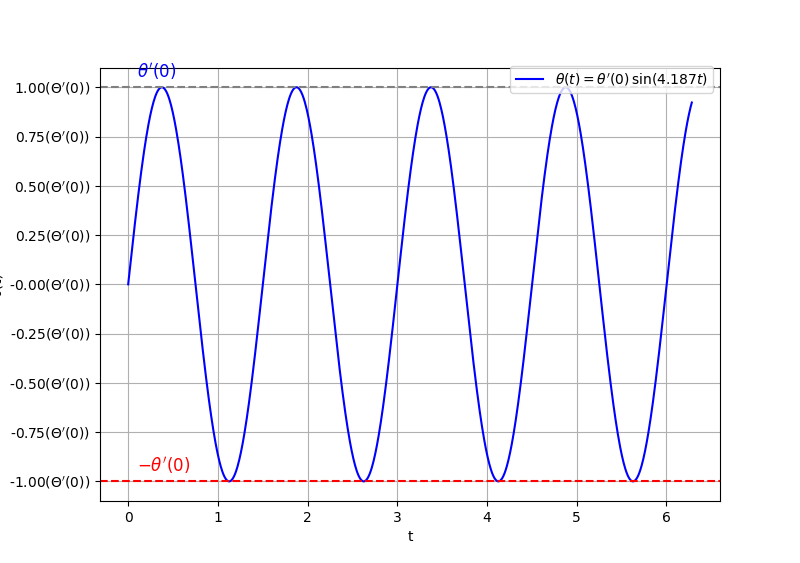
\includegraphics[width=\columnwidth]{graph_1}
\caption{ $\theta(t)$ vs t }
\label{graph:ee25-analog graph}
\end{figure}

\pagebreak
\item Suppose that the electric field amplitude of an electromagnetic wave is $E_0$ = 120N/C and that its frequency is $f$ = 50.0 MHz.
\begin{enumerate} [label=(\alph*)]
    \item Determine, $B_0, \omega, k$ and $\lambda$
    \item Find expressions for \textbf{E} and \textbf{B}
\end{enumerate}
\solution
\iffalse
\let\negmedspace\undefined
\let\negthickspace\undefined
\documentclass[journal,12pt,twocolumn]{IEEEtran}
\usepackage{cite}
\usepackage{amsmath,amssymb,amsfonts,amsthm}
\usepackage{algorithmic}
\usepackage{graphicx}

\usepackage{textcomp}
\usepackage{xcolor}
\usepackage{txfonts}
\usepackage{listings}
\usepackage{enumitem}
\usepackage{mathtools}
\usepackage{gensymb}
\usepackage{comment}
\usepackage[breaklinks=true]{hyperref}
\usepackage{tkz-euclide} 
\usepackage{listings}
\usepackage{gvv}                                                                      
\usepackage[latin1]{inputenc}                                
\usepackage{color}                                            
\usepackage{array}                                            
\usepackage{longtable}                                       
\usepackage{calc}                                             
\usepackage{multirow}                                         
\usepackage{hhline}                                           
\usepackage{ifthen}                                           
\usepackage{lscape}
\setlength{\arrayrulewidth}{0.5mm}
\setlength{\tabcolsep}{18pt}
\renewcommand{\arraystretch}{1.5}
\newtheorem{theorem}{Theorem}[section]
\newtheorem{problem}{Problem}
\newtheorem{proposition}{Proposition}[section]
\newtheorem{lemma}{Lemma}[section]
\newtheorem{corollary}[theorem]{Corollary}
\newtheorem{example}{Example}[section]
\newtheorem{definition}[problem]{Definition}
\newcommand{\BEQA}{\begin{eqnarray}}
\newcommand{\EEQA}{\end{eqnarray}}
\newcommand{\define}{\stackrel{\triangle}{=}}
\theoremstyle{remark}
\newtheorem{rem}{Remark}

\begin{document}

\bibliographystyle{IEEEtran}
\vspace{3cm}

\title{NCERT 12.8 8}
\author{EE23BTECH11054 - Sai Krishna Shanigarapu% <-this % stops a space
}
\maketitle
\newpage
\bigskip

\begin{flushleft}
\textbf{Question 8}\\
Suppose that the electric field amplitude of an electromagnetic wave is $E_0$ = 120N/C and that its frequency is $f$ = 50.0 MHz.\\
(a) Determine, $B_0, \omega, k$ and $\lambda$\\
(b) Find expressions for \textbf{E} and \textbf{B}\\
\end{flushleft}

\bigskip


Solution:
\fi

\begin{center}
    \begin{table}[ht]
        \caption{Input Parameters}
        \setlength{\arrayrulewidth}{0.3mm}
\setlength{\tabcolsep}{15pt}
\renewcommand{\arraystretch}{1.5}

%\textbf{Table 1}\\
\begin{center}
\begin{tabular}{ |p{1cm}|p{2.5cm}|p{1.7cm}|  }

\hline
Symbol& Description&value\\
\hline
$f$ & frequency of source & 50.0 MHz\\
\hline
$E_0$ & Electric field amplitude  & 120 N/C\\
\hline
$c$ &speed of light & 3 x 10$^8$ m/s \\
\hline
$\vec{e_2}, \vec{e_3}$ & Standard Basis vectors & N/A\\
\hline

\end{tabular}
\end{center}
        \label{tab:table1.12.8.8}
    \end{table}
\end{center}


\begin{flushleft}
    \begin{table}[ht]
       \caption{Formulae and Output}
       \setlength{\arrayrulewidth}{0.3mm}
\setlength{\tabcolsep}{15pt}
\renewcommand{\arraystretch}{1.5}

%\textbf{Table 1}\\
\begin{center}
\begin{tabular}{ |p{1cm}|p{2.5cm}|p{1.7cm}|  }

\hline
Symbol& Description&value\\
\hline
$f$ & frequency of source & 50.0 MHz\\
\hline
$E_0$ & Electric field amplitude  & 120 N/C\\
\hline
$c$ &speed of light & 3 x 10$^8$ m/s \\
\hline
$\vec{e_2}, \vec{e_3}$ & Standard Basis vectors & N/A\\
\hline

\end{tabular}
\end{center}
       \label{tab:table2.12.8.8}
    \end{table}
\bigskip
\end{flushleft}

\bigskip


\newpage
\renewcommand{\thefigure}{\theenumi}
\renewcommand{\thetable}{\theenumi}

\begin{flushleft}

\begin{figure}[h]
\renewcommand\thefigure{1}
  \caption{Graphs of $\vec{E} \text{ and } \vec{B}$}
  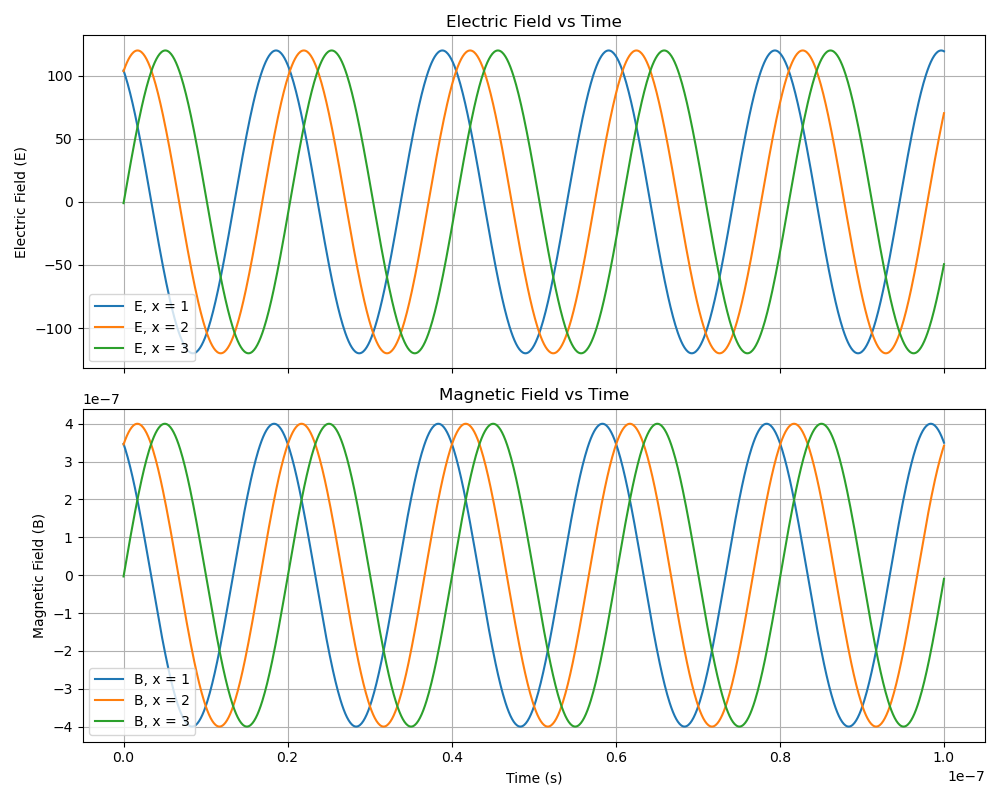
\includegraphics[width=1.05\columnwidth]{ncert-physics/12/8/8/figs/Figure_1.png}
  \label{fig:fig1.12.8.8}

\end{figure}

\end{flushleft}

%\end{document}


\pagebreak
\item A charged particle oscillates about its mean equilibrium position with a frequency of $10^9Hz$. What is the frequency of the electromagnetic waves produced by the oscillator? \\
\solution
\iffalse
\let\negmedspace\undefined
\let\negthickspace\undefined
\documentclass[journal,12pt,twocolumn]{IEEEtran}
\usepackage{cite}
\usepackage{amsmath,amssymb,amsfonts,amsthm}
\usepackage{algorithmic}
\usepackage{graphicx}
\usepackage{textcomp}
\usepackage{xcolor}
\usepackage{txfonts}
\usepackage{listings}
\usepackage{enumitem}
\usepackage{mathtools}
\usepackage{gensymb}
\usepackage{comment}
\usepackage[breaklinks=true]{hyperref}
\usepackage{tkz-euclide} 
\usepackage{listings}
\usepackage{gvv}                                        
\def\inputGnumericTable{}                                 
\usepackage[latin1]{inputenc}                                
\usepackage{color}                                            
\usepackage{array}                                            
\usepackage{longtable}                                       
\usepackage{calc}                                             
\usepackage{multirow}                                         
\usepackage{hhline}                                           
\usepackage{ifthen}                                           
\usepackage{lscape}
\usepackage[export]{adjustbox}

\newtheorem{theorem}{Theorem}[section]
\newtheorem{problem}{Problem}
\newtheorem{proposition}{Proposition}[section]
\newtheorem{lemma}{Lemma}[section]
\newtheorem{corollary}[theorem]{Corollary}
\newtheorem{example}{Example}[section]
\newtheorem{definition}[problem]{Definition}
\newcommand{\BEQA}{\begin{eqnarray}}
\newcommand{\EEQA}{\end{eqnarray}}
\newcommand{\define}{\stackrel{\triangle}{=}}
\theoremstyle{remark}
\newtheorem{rem}{Remark}
\begin{document}
\parindent 0px
\bibliographystyle{IEEEtran}

\title{Assignment\\[1ex]12.8 - 6}
\author{EE23BTECH11034 - Prabhat Kukunuri$^{}$% <-this % stops a space
}
\maketitle
\newpage
\bigskip

\renewcommand{\thefigure}{\theenumi}
\renewcommand{\thetable}{\theenumi}
\section*{Question}
A charged particle oscillates about its mean equilibrium position with a frequency of $10^9Hz$. What is the frequency of the electromagnetic waves produced by the oscillator?

\section*{Solution}
\fi
\begin{table}[h]
    \centering
    \begin{tabular}{|c|c|c|}
    \hline
   Symbol&Value&Description\\ \hline
   $y(t)$&$\cos\brak{2{\pi}f_ct}$&Wave equation of electro-magnetic wave\\ \hline
   $f_c$&$10^9$&Frequency of electromagnetic wave\\ \hline
   $t$&seconds&Time\\ \hline

    \end{tabular}
    \caption{Variable description}
    \label{tab:12.8.6.1}
\end{table}

\begin{figure}[h]
    \centering
    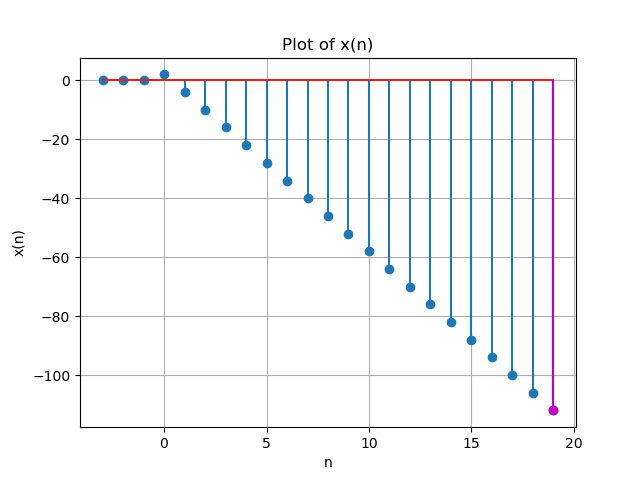
\includegraphics[width=\columnwidth]{Figure_1.png}
    \caption{$y(t)=\cos\brak{2{\pi}\times 10^9t}$}
    \label{fig:12.8.6.2}
\end{figure}
%\end{document}
\pagebreak
\item Given below are some functions of x and t to 
represent the displacement (transverse
or longitudinal) of an elastic wave. State which of these represents \brak i travelling
wave, \brak {ii} a stationary wave or \brak {iii} none at all: \\
\begin{enumerate}
\item $y = 2\cos \brak{3x} \sin \brak{10t}$
\item $y=2\sqrt{x-vt}$
\item $y = 3\sin \brak{5x - 0.5t} + 4\cos \brak{5x - 0.5t}$
\item $y = \cos x \sin t + \cos 2x \sin 2t$
\end{enumerate}
\solution
\iffalse
\let\negmedspace\undefined
\let\negthickspace\undefined
\documentclass[journal,12pt,twocolumn]{IEEEtran}
\usepackage{cite}
\usepackage{amsmath,amssymb,amsfonts,amsthm}
\usepackage{algorithmic}
\usepackage{graphicx}
\usepackage{textcomp}
\usepackage{xcolor}
\usepackage{txfonts}
\usepackage{listings}
\usepackage{enumitem}
\usepackage{mathtools}
\usepackage{gensymb}
\usepackage{comment}
\usepackage[breaklinks=true]{hyperref}
\usepackage{tkz-euclide} 
\usepackage{listings}
\usepackage{gvv}                                        
\def\inputGnumericTable{}                                 
\usepackage[latin1]{inputenc}                                
\usepackage{color}                                            
\usepackage{array}                                            
\usepackage{longtable}                                       
\usepackage{calc}                                             
\usepackage{multirow}                                         
\usepackage{hhline}                                           
\usepackage{ifthen}                                           
\usepackage{lscape}
\newtheorem{theorem}{Theorem}[section]
\newtheorem{problem}{Problem}
\newtheorem{proposition}{Proposition}[section]
\newtheorem{lemma}{Lemma}[section]
\newtheorem{corollary}[theorem]{Corollary}
\newtheorem{example}{Example}[section]
\newtheorem{definition}[problem]{Definition}
\newcommand{\BEQA}{\begin{eqnarray}}
\newcommand{\EEQA}{\end{eqnarray}}
\newcommand{\define}{\stackrel{\triangle}{=}}
\theoremstyle{remark}
\newtheorem{rem}{Remark}
\begin{document}
\parindent 0px
\bibliographystyle{IEEEtran}
\title{ASSIGNMENT11.15\_13Q}
\author{EE22BTECH11219 - Sai Sujan Rada$^{}$% <-this % stops a space
}
\maketitle
\newpage
\bigskip
\section*{QUESTION}
Given below are some functions of x and t to 
represent the displacement (transverse
or longitudinal) of an elastic wave. State which of these represents \brak i travelling
wave, \brak {ii} a stationary wave or \brak {iii} none at all: \\
\begin{enumerate}
\item $y = 2\cos \brak{3x} \sin \brak{10t}$
\item $y=2\sqrt{x-vt}$
\item $y = 3\sin \brak{5x - 0.5t} + 4\cos \brak{5x - 0.5t}$
\item $y = \cos x \sin t + \cos 2x \sin 2t$
\end{enumerate}
\solution 

\fi
\begin{table}[htbp]
    \centering
    \def\arraystretch{1.5}
    \begin{tabular}{|p{4cm}|p{4cm}|}
    \hline
TRAVELLING WAVE  & STATIONARY WAVE \\ \hline
    $y \brak{x,t} =A \sin  \brak{kx \pm \omega t} $ & $y\brak{ x,t }=A\sin kx\cos \omega t $ \\   \hline
    \hline
PARAMETERS  & DEFINITION  \\  \hline
$A$    &  Amplitude  \\ \hline
 $\omega$  & Angular Velocity  \\  \hline
 $x$    & Position  \\  \hline
 $k$    & Wavenumber    \\  \hline 
    \end{tabular}
    \caption{Travelling wave $vs$ Stationary wave}
    \label{tab:table11.15.13.1}
\end{table}

Let us assume an equation:
\begin{align}
y=A(x)\cos \brak{\omega t+\phi\brak {x}}
\end{align}
\begin{table}[htbp]
    \centering
    \def\arraystretch{1.5}
    \begin{tabular}{|p{4cm}|p{4cm}|}
    \hline
STATIONARY WAVE CONDITION & TRAVELLING WAVE CONDITION \\ \hline
        \brak 1 $A(x)$ should be a function of position x, and it can be expressed as $A(x)=A_{0}cos(\omega t+\alpha)$ where $A_{0}$ is a constant, $k$ is the wavenumber, $x$ is the position and $\alpha$ is a phase constant. & 
        \brak 1 $A(x)$ should be a constant, and it can be expressed as $A(x)=A_{0}$ where $A_{0}$ is a constant number. \\ \hline

        \brak 2 $\phi (x)$ can be expressed as $\phi (x)=c$ where c is a constant. &
        \brak 2 $\phi (x)$ represents a linear expression in x, and it can be expressed as $\phi (x)=kx+\theta$ where k is the wavenumber and $\theta$ is the phaseconstant. \\ \hline
\end{tabular}
    \caption{Travelling wave $vs$ Stationary wave}
    \label{tab:table1}
\end{table}

\begin{figure}[ht]
                        \centering
                        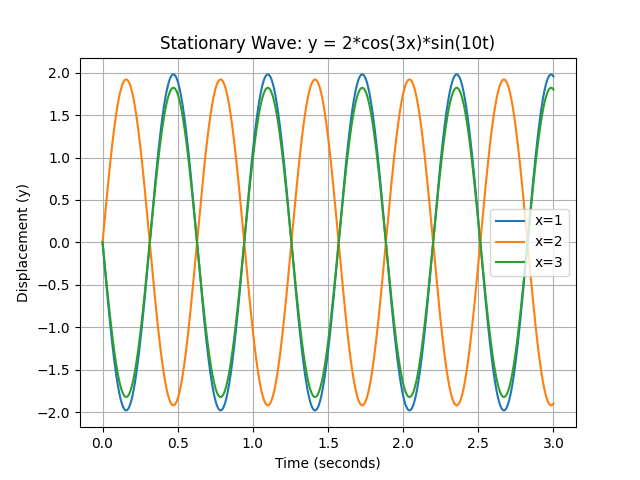
\includegraphics[width=\columnwidth]{figs/a.png}
                        \caption{DIPLACEMENT $vs$ TIME-graph1}
                        \label{fig:11.15.13.1}
\end{figure}
\begin{figure}[ht]
                            \centering
                            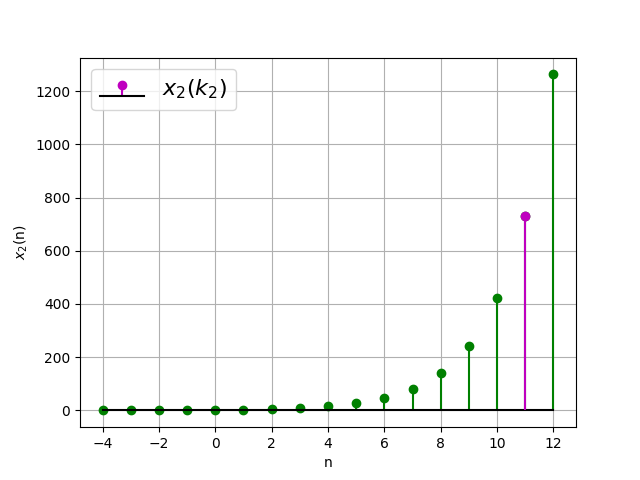
\includegraphics[width=\columnwidth]{figs/b.png}
                            \caption{DIPLACEMENT $vs$ TIME-graph2}
                            \label{fig:11.15.13.2}
\end{figure}   
\begin{figure}[ht]
                             \centering
                             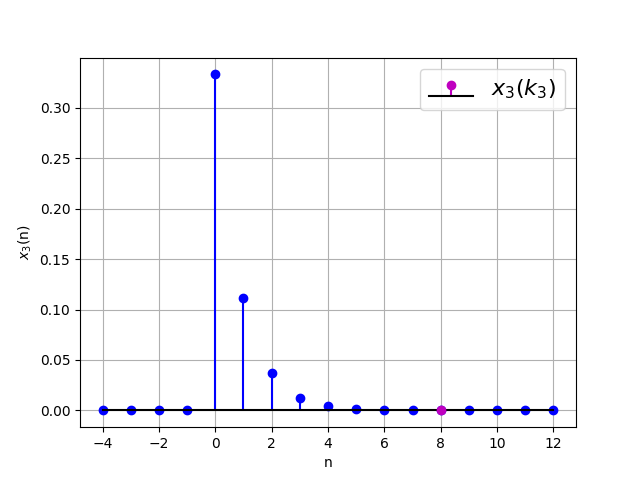
\includegraphics[width=\columnwidth]{figs/c.png}
                             \caption{DIPLACEMENT $vs$ TIME-graph3}
                             \label{fig:11.15.13.3}
\end{figure}
\begin{figure}[ht]
                            \centering
                            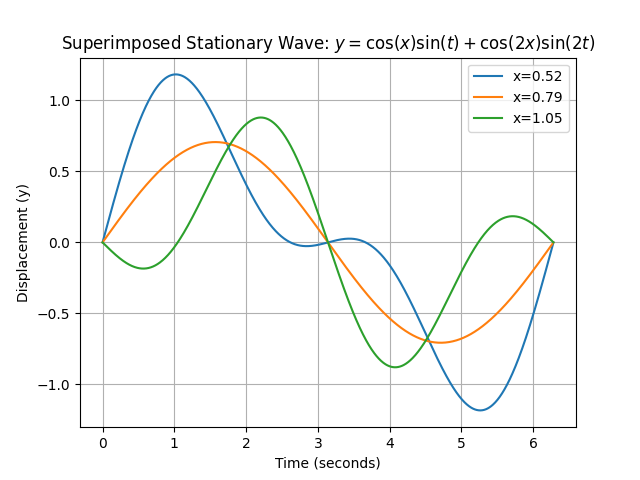
\includegraphics[width=\columnwidth]{figs/d.png}
                            \caption{DIPLACEMENT $vs$ TIME-graph4}
                            \label{fig:11.15.13.4}
\end{figure}
\figref{fig:11.15.13.1} and \figref{fig:11.15.13.3} are self explanatory for stationary and travelling waves.\figref{fig:11.15.13.2} and \figref{fig:11.15.13.4} are neither stationary nor travelling waves.


\pagebreak
\item For the travelling harmonic wave
$y\brak {x, t} = 2.0 \cos 2\pi \brak{10t - 0.0080 x + 0.35}$ where $x$ and $y$ are in $cm$ and $t$ in $s$. Calculate the phase difference between oscillatory
motion of two points separated by a distance of 

\begin{enumerate} [label=(\alph*)]
    \item $4 m$
    \item $0.5 m$
    \item $\lambda/2$
    \item $3\lambda/4$
\end{enumerate}
\solution
% \iffalse
\let\negmedspace\undefined
\let\negthickspace\undefined
\documentclass[journal,12pt,twocolumn]{IEEEtran}
\usepackage{cite}
\usepackage{amsmath,amssymb,amsfonts,amsthm}
\usepackage{algorithmic}
\usepackage{graphicx}
\usepackage{textcomp}
\usepackage{xcolor}
\usepackage{txfonts}
\usepackage{listings}
\usepackage{enumitem}
\usepackage{mathtools}
\usepackage{gensymb}
\usepackage{comment}
\usepackage[breaklinks=true]{hyperref}
\usepackage{tkz-euclide} 
\usepackage{listings}
\usepackage{gvv}                                        
\def\inputGnumericTable{}                                 
\usepackage[latin1]{inputenc}                               \usepackage{caption}
\usepackage{color}                                            
\usepackage{array}                                            
\usepackage{longtable}                                       
\usepackage{calc}                                             
\usepackage{multirow}                                         
\usepackage{hhline}                                           
\usepackage{ifthen}                                           
\usepackage{lscape}

\newtheorem{theorem}{Theorem}[section]
\newtheorem{problem}{Problem}
\newtheorem{proposition}{Proposition}[section]
\newtheorem{lemma}{Lemma}[section]
\newtheorem{corollary}[theorem]{Corollary}
\newtheorem{example}{Example}[section]
\newtheorem{definition}[problem]{Definition}
\newcommand{\BEQA}{\begin{eqnarray}}
\newcommand{\EEQA}{\end{eqnarray}}
\newcommand{\define}{\stackrel{\triangle}{=}}
\theoremstyle{remark}
\newtheorem{rem}{Remark}
\begin{document}

\bibliographystyle{IEEEtran}
\vspace{3cm}

\title{NCERT 11.15. Q10}
\author{EE23BTECH11010 - Venkatesh Bandawar$^{*}$% <-this % stops a space
}
\maketitle
\newpage
\bigskip

\renewcommand{\thefigure}{\arabic{figure}}
\renewcommand{\thetable}{\arabic{table}}

\bibliographystyle{IEEEtran}

\parindent 0px
\textbf{Question:} For the travelling harmonic wave
$y\brak {x, t} = 2.0 \cos 2\pi \brak{10t - 0.0080 x + 0.35}$ where $x$ and $y$ are in $cm$ and $t$ in $s$. Calculate the phase difference between oscillatory
motion of two points separated by a distance of 

\begin{enumerate} [label=(\alph*)]
    \item $4 m$
    \item $0.5 m$
    \item $\lambda/2$
    \item $3\lambda/4$
\end{enumerate}

\textbf{Solution:}  
\begin{table}[htbp] \small
\centering
\begin{table}[ht]
    \centering
    \begin{tabular}{|c|c|c|}
        \hline
        Parameter & Value & Description \\
        \hline
        $x(0)$ & 5 & First term of AP \\
        $d$ & 1.75 & Common difference of AP \\
        $x(n)$ & 20.75 & $n^{th}$ term of AP \\
        \hline
    \end{tabular}
    \vspace{2mm}
    \caption{Parameter List}
    \label{tab:simple.10.5.2.20}
\end{table}

\caption{Given \, parameters list}
\label{tab:given parameters list}
\end{table}
\begin{align}
    \brak{\Delta \theta} &= \brak{ 2\pi f t - kx_1 + \phi}  - \brak{2\pi f t -kx_2 + \phi}\\
    &= k\brak{x_2 - x_1} 
\end{align}

\begin{table}[htbp] 
\centering
\begin{tabular}{|c|c|c|}
        \hline
        \textbf{Parameter} & \textbf{Value} & \textbf{Description} \\
        \hline
        $x(0)$ & & First term \\
        \hline
        $r$ & & Common ratio \\
        \hline
        $x(0)^3r^3$ & 1 & Product of terms \\
        \hline
        $x(0)$ + $x(0)r$ + $x(0)r^2$ & $\frac{39}{10}$ & Sum of terms \\
        \hline
    \end{tabular}

\caption{Phase \, differences}
\label{tab:phase differences}
\end{table}

\begin{figure}[!h] 
\centering
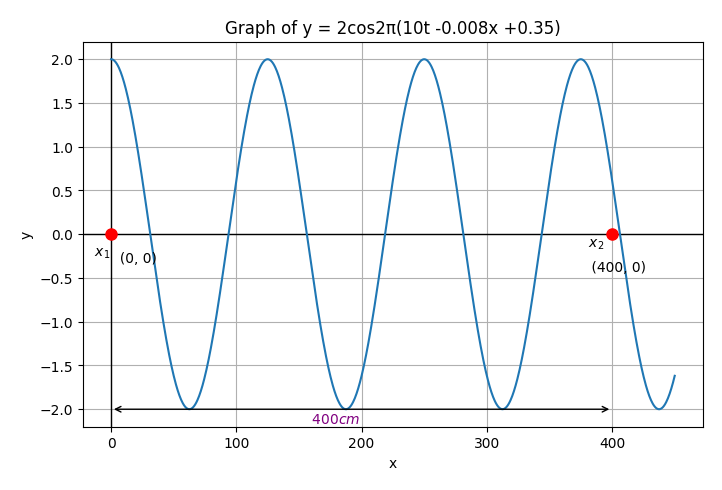
\includegraphics[width=\columnwidth]{figs/graph1.png}
\captionsetup{justification=centering}
\caption{}
\label{fig:Graph1}
\end{figure}

\begin{figure}[!h] 
\centering
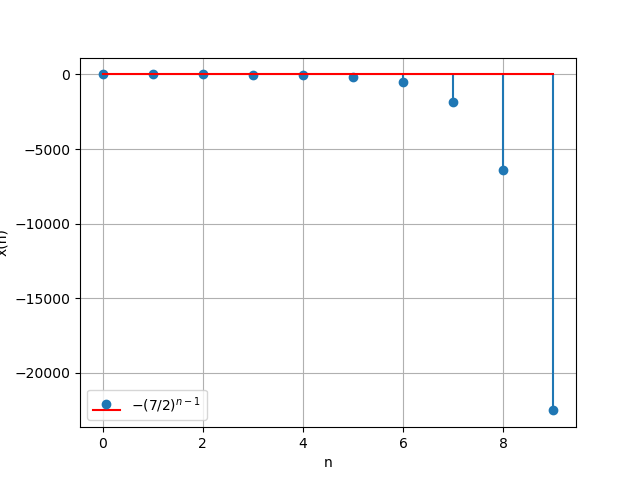
\includegraphics[width=\columnwidth]{figs/graph2.png}
\captionsetup{justification=centering}
\caption{}
\label{fig:Graph2}
\end{figure}

\begin{figure}[!h] 
\centering
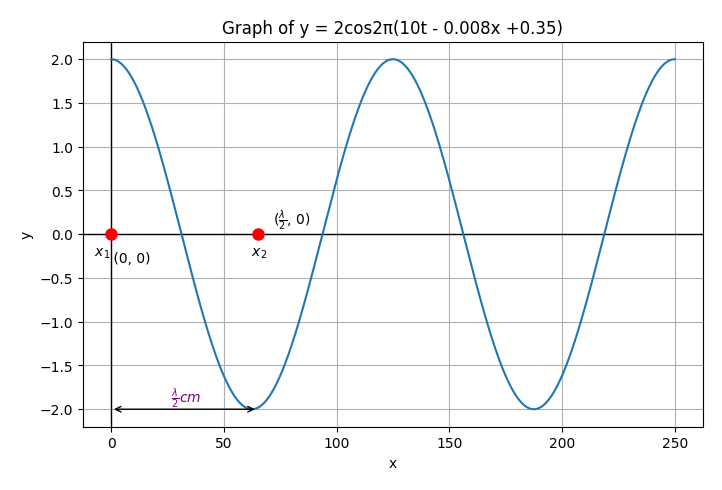
\includegraphics[width=\columnwidth]{figs/graph3.png}
\captionsetup{justification=centering}
\caption{}
\label{fig:Graph3}
\end{figure}

\begin{figure}[!h] 
\centering
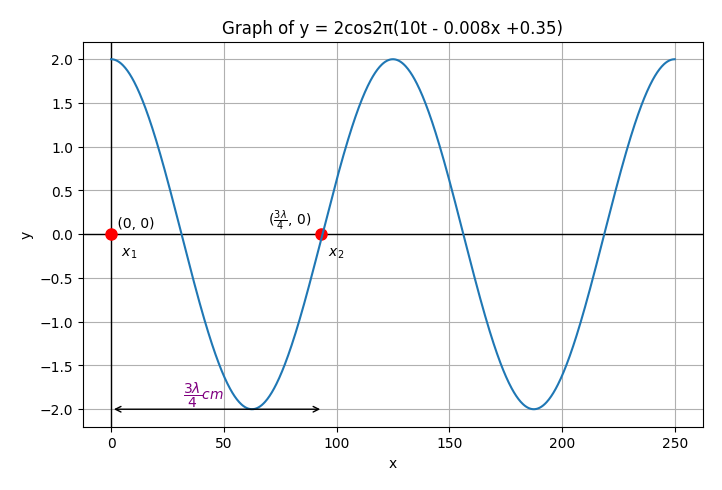
\includegraphics[width=\columnwidth]{figs/graph4.png}
\captionsetup{justification=centering}
\caption{}
\label{fig:Graph4}
\end{figure}



\end{document}

\pagebreak
\item 
\begin{enumerate}
\item The peak voltage of an AC supply is 300 V. What is the rms voltage?
\item The rms value of current in an AC circuit is 10 A. What is the peak current?
\end{enumerate}
\solution
\iffalse
\let\negmedspace\undefined
\let\negthickspace\undefined
\documentclass[journal,12pt,onecolumn]{IEEEtran}
\usepackage{cite}
\usepackage{amsmath,amssymb,amsfonts,amsthm}
%\usepackage{algorithmic}
\usepackage{graphicx}
\usepackage{textcomp}
usepackage{array}
\usepackage{xcolor}
\usepackage{txfonts}
\usepackage{listings}
\usepackage{enumitem}
\usepackage{mathtools}
\usepackage{gensymb}
\usepackage[breaklinks=true]{hyperref}
\usepackage{tkz-euclide} % loads  TikZ and tkz-base
\usepackage{listings}
\usepackage{float}



\newtheorem{theorem}{Theorem}[section]
\newtheorem{problem}{Problem}
\newtheorem{proposition}{Proposition}[section]
\newtheorem{lemma}{Lemma}[section]
\newtheorem{corollary}[theorem]{Corollary}
\newtheorem{example}{Example}[section]
\newtheorem{definition}[problem]{Definition}
%\newtheorem{thm}{Theorem}[section] 
%\newtheorem{defn}[thm]{Definition}
%\newtheorem{algorithm}{Algorithm}[section]
%\newtheorem{cor}{Corollary}
\newcommand{\BEQA}{\begin{eqnarray}}
\newcommand{\EEQA}{\end{eqnarray}}
\newcommand{\define}{\stackrel{\triangle}{=}}
\theoremstyle{remark}
\newtheorem{rem}{Remark}
%\bibliographystyle{ieeetr}
\begin{document}
%
\providecommand{\pr}[1]{\ensuremath{\Pr\left(#1\right)}}
\providecommand{\prt}[2]{\ensuremath{p_{#1}^{\left(#2\right)} }}        % own macro for this question
\providecommand{\qfunc}[1]{\ensuremath{Q\left(#1\right)}}
\providecommand{\sbrak}[1]{\ensuremath{{}\left[#1\right]}}
\providecommand{\lsbrak}[1]{\ensuremath{{}\left[#1\right.}}
\providecommand{\rsbrak}[1]{\ensuremath{{}\left.#1\right]}}
\providecommand{\brak}[1]{\ensuremath{\left(#1\right)}}
\providecommand{\lbrak}[1]{\ensuremath{\left(#1\right.}}
\providecommand{\rbrak}[1]{\ensuremath{\left.#1\right)}}
\providecommand{\cbrak}[1]{\ensuremath{\left\{#1\right\}}}
\providecommand{\lcbrak}[1]{\ensuremath{\left\{#1\right.}}
\providecommand{\rcbrak}[1]{\ensuremath{\left.#1\right\}}}
\newcommand{\sgn}{\mathop{\mathrm{sgn}}}
\providecommand{\abs}[1]{\left\vert#1\right\vert}
\providecommand{\res}[1]{\Res\displaylimits_{#1}} 
\providecommand{\norm}[1]{\left\lVert#1\right\rVert}
%\providecommand{\norm}[1]{\lVert#1\rVert}
\providecommand{\mtx}[1]{\mathbf{#1}}
\providecommand{\mean}[1]{E\left[ #1 \right]}
\providecommand{\cond}[2]{#1\middle|#2}
\providecommand{\fourier}{\overset{\mathcal{F}}{ \rightleftharpoons}}
\newenvironment{amatrix}[1]{%
  \left(\begin{array}{@{}*{#1}{c}|c@{}}
}{%
  \end{array}\right)
}
%\providecommand{\hilbert}{\overset{\mathcal{H}}{ \rightleftharpoons}}
%\providecommand{\system}{\overset{\mathcal{H}}{ \longleftrightarrow}}
	%\newcommand{\solution}[2]{\textbf{Solution:}{#1}}
\newcommand{\solution}{\noindent \textbf{Solution: }}
\newcommand{\cosec}{\,\text{cosec}\,}
\providecommand{\dec}[2]{\ensuremath{\overset{#1}{\underset{#2}{\gtrless}}}}
\newcommand{\myvec}[1]{\ensuremath{\begin{pmatrix}#1\end{pmatrix}}}
\newcommand{\mydet}[1]{\ensuremath{\begin{vmatrix}#1\end{vmatrix}}}
\newcommand{\myaugvec}[2]{\ensuremath{\begin{amatrix}{#1}#2\end{amatrix}}}
\providecommand{\rank}{\text{rank}}
\providecommand{\pr}[1]{\ensuremath{\Pr\left(#1\right)}}
\providecommand{\qfunc}[1]{\ensuremath{Q\left(#1\right)}}
	\newcommand*{\permcomb}[4][0mu]{{{}^{#3}\mkern#1#2_{#4}}}
\newcommand*{\perm}[1][-3mu]{\permcomb[#1]{P}}
\newcommand*{\comb}[1][-1mu]{\permcomb[#1]{C}}
\providecommand{\qfunc}[1]{\ensuremath{Q\left(#1\right)}}
\providecommand{\gauss}[2]{\mathcal{N}\ensuremath{\left(#1,#2\right)}}
\providecommand{\diff}[2]{\ensuremath{\frac{d{#1}}{d{#2}}}}
\providecommand{\myceil}[1]{\left \lceil #1 \right \rceil }
\newcommand\figref{Fig.~\ref}
\newcommand\tabref{Table~\ref}
\newcommand{\sinc}{\,\text{sinc}\,}
\newcommand{\rect}{\,\text{rect}\,}
%%
%	%\newcommand{\solution}[2]{\textbf{Solution:}{#1}}
%\newcommand{\solution}{\noindent \textbf{Solution: }}
%\newcommand{\cosec}{\,\text{cosec}\,}
%\numberwithin{equation}{section}
%\numberwithin{equation}{subsection}
%\numberwithin{problem}{section}
%\numberwithin{definition}{section}
%\makeatletter
%\@addtoreset{figure}{problem}
%\makeatother

%\let\StandardTheFigure\thefigure
\let\vec\mathbf

\bibliographystyle{IEEEtran}





\bigskip

%\renewcommand{\thefigure}{\theenumi}
%\renewcommand{\thetable}{\theenumi}
%\renewcommand{\theequation}{\theenumi}

Q: \\
\begin{enumerate}
\item The peak voltage of an AC supply is 300 V. What is the rms voltage?
\item The rms value of current in an AC circuit is 10 A. What is the peak current?
\end{enumerate}

\solution
\fi

\begin{table}
\centering
  \begin{tabular}{|c|c|c|}
    \hline
    parameter & value & description \\
    \hline
    $V(t)$ & $V_{\text{0}} \cdot \sin(2\pi ft + \phi)$ & voltage in terms of time \\
    \hline
    $I(t)$ & $I_{\text{0}} \cdot \sin(2\pi ft + \phi)$ & current in terms of time \\
    \hline
    $V_0$ & $300 \, \text{V}$ & peak voltage \\
    \hline
    $V_ \text{rms}$ & $\sqrt{\frac{1}{T} \int_{0}^{T} [V(t)]^2 \, dt}$ & rms value of Voltage \\
    \hline 
    $I_ \text{rms}$ & $10 \, \text{A}$ & rms value of current\\
    \hline
    $I_0$ & $\sqrt{2} \times I_{\text{rms}}$ & peak current \\
    \hline
    $f$ & $50 \, \text{Hz}$ & frequence of the sinosoidal wave. \\
    \hline
    $T$ & $0.02 \, \text{s}$ & time period of sinosoidal wave. \\
    \hline
  \end{tabular}

\caption{Input Parameter Table}
\label{tab:input_parameters}
\end{table}
  


\begin{enumerate}
\item
\begin{align}
V_{\text{rms}}^2 &= {\frac{1}{T} \int_{0}^{T} [V(t)]^2 \, dt} \\
&= {f \int_{0}^{\frac{1}{f}} V_{\text{0}}^2 \cdot \sin^2(2\pi ft + \phi) \, dt} \\
&= \frac{1}{2} V_{0}^2 \left(1 - \frac{1}{f}\int_{0}^{\frac{1}{f}} \cos(4\pi ft + 2\phi) \, dt \right) \\
&= \frac{1}{2} V_{0}^2 \left(1 - \frac{1}{f}\left[\frac{\sin(4\pi ft + 2\phi)}{4\pi f}\right]_{0}^{\frac{1}{f}}\right) \\
&= \frac{1}{2} V_{0}^2 \left(1 - \frac{1}{f} \cdot \frac{\sin\left(4\pi + 2\phi\right) - \sin(0 + 2\phi)}{4\pi f}\right) \\
V_{\text{rms}} &= \frac{V_{0}}{\sqrt{2}} \label{eq:12.7.2_voltage}
\end{align}

To find the RMS voltage (\(V_{\text{rms}})\) when the peak voltage (\(V_{\text{0}})\) is 300V, you can use equation  \eqref{eq:12.7.2_voltage}

\begin{align}
V_{\text{rms}} &= \frac{300V}{\sqrt{2}} \approx 212.13V
\end{align}

\item 
\begin{align}
I_{\text{rms}}^2 &= {\frac{1}{T} \int_{0}^{T} [I(t)]^2 \, dt} \\
&= {f \int_{0}^{\frac{1}{f}} I_{\text{0}}^2 \cdot \sin^2(2\pi ft + \phi) \, dt} \\
&= \frac{1}{2} I_{0}^2 \left(1 - \frac{1}{f}\left[\frac{\sin(4\pi ft + 2\phi)}{4\pi f}\right]_{0}^{\frac{1}{f}}\right) \\
&= \frac{1}{2} I_{0}^2 \left(1 - \frac{1}{f} \cdot \frac{\sin\left(4\pi + 2\phi\right) - \sin(0 + 2\phi)}{4\pi f}\right) \\
I_{\text{rms}} &= \frac{I_{0}}{\sqrt{2}} \label{eq:12.7.2_current}
\end{align}

To find the peak current (\(I_{\text{0}}\)) when the RMS current (\(I_{\text{rms}}\)) is given, you can use equation  \eqref{eq:12.7.2_current}

\begin{align}
I_{\text{0}} \approx 10 \, \text{A} \times 1.414 \approx 14.14 \, \text{A}  
\end{align}

\begin{figure}[H]
    \centering
    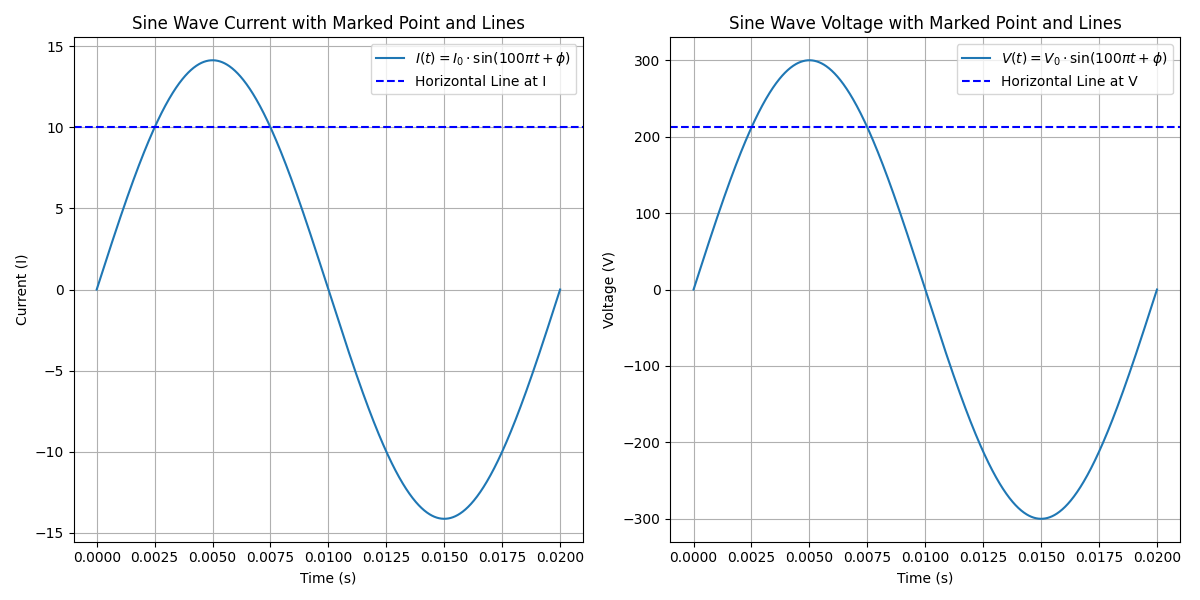
\includegraphics[width=\columnwidth]{.figs/merged_sine_wave_plots.png}

\end{enumerate}


\pagebreak
\item In Young’s double-slit experiment using monochromatic light of wavelength $\lambda$, the intensity of light at a point on the screen where path difference is $\lambda$, is $K$ units. What is the intensity of light at a
point where path difference is $\lambda$/3?\\

\solution

% \iffalse
\let\negmedspace\undefined
\let\negthickspace\undefined
\documentclass[journal,12pt,twocolumn]{IEEEtran}
\usepackage{cite}
\usepackage{amsmath,amssymb,amsfonts,amsthm}
\usepackage{algorithmic}
\usepackage{graphicx}
\usepackage{textcomp}
\usepackage{xcolor}
\usepackage{txfonts}
\usepackage{listings}
\usepackage{enumitem}
\usepackage{mathtools}
\usepackage{gensymb}
\usepackage{comment}
\usepackage[breaklinks=true]{hyperref}
\usepackage{tkz-euclide} 
\usepackage{listings}
\usepackage{gvv} 
\usepackage{caption}
\def\inputGnumericTable{}                                 
%\usepackage[latin1]{inputenc}                                
\usepackage{color}                                            
\usepackage{array}                                            
\usepackage{longtable}                                       
\usepackage{calc}                                             
\usepackage{multirow}                                         
\usepackage{hhline}                                           
\usepackage{ifthen}                                           
\usepackage{lscape}

\newtheorem{theorem}{Theorem}[section]
\newtheorem{problem}{Problem}
\newtheorem{proposition}{Proposition}[section]
\newtheorem{lemma}{Lemma}[section]
\newtheorem{corollary}[theorem]{Corollary}
\newtheorem{example}{Example}[section]
\newtheorem{definition}[problem]{Definition}
\newcommand{\BEQA}{\begin{eqnarray}}
\newcommand{\EEQA}{\end{eqnarray}}
\newcommand{\define}{\stackrel{\triangle}{=}}
\theoremstyle{remark}
\newtheorem{rem}{Remark}

\begin{document}

\bibliographystyle{IEEEtran}
\vspace{3cm}

\title{NCERT 12.10 5Q}
\author{EE23BTECH11013 - Avyaaz$^{*}$% <-this % stops a space 
}
\maketitle
\newpage
\bigskip

\renewcommand{\thefigure}{\arabic{figure}}
\renewcommand{\thetable}{\arabic{table}}

\large\textbf{\textsl{Question:}}
In Young’s double-slit experiment using monochromatic light of wavelength $\lambda$, the intensity of light at a point on the screen where path difference is $\lambda$, is $K$ units. What is the intensity of light at a
point where path difference is $\lambda$/3?\\
\large\textbf{\textsl{Solution:}}
\begin{table}[htbp]
\setlength{\extrarowheight}{8pt}
\centering
\begin{table}[h]
\renewcommand\thetable{1}
    \centering
    \begin{tabular}{|c|c|c|}
        \hline
        \textbf{Parameter} & \textbf{Description} & \textbf{Value}\\
        \hline
        $x(0)$ & First term & $2$\\
        \hline
        $x(19)$ & $20\textsuperscript{th}$ term & $-112$\\
        \hline
        $y(n)$ & sum upto $n\textsuperscript{th}$ term & \\
        \hline
    \end{tabular}
    \caption{Input data}
  \label{input data}
\end{table}

\caption{Parameters}
\label{tab:parameters}
\end{table}

From \tabref{tab:parameters}:
\begin{align}
%%y\brak{t} &= y_1\brak{t} + y_2\brak{t}  \\
y\brak{t} &= A\sin({2\pi f t - kx_1})  + A\sin({ 2\pi f t - kx_2}) \\
y\brak{t} &=  2A\cos\left(\dfrac{k\Delta x}{2}\right)\sin\left(2\pi f t - \dfrac{k(x_1+x_2)}{2} \right) \label{eq:superposition}
\end{align}
From \tabref{tab:parameters} and equation \eqref{eq:superposition}: 
\begin{align}
\therefore I \propto 4A^2\cos^2\left(\dfrac{k\Delta x}{2}\right)  \label{eq:intensity}
\end{align}
From \tabref{tab:parameters} and equation \eqref{eq:intensity}: 
\begin{align}
 \dfrac{K}{I_r} = \dfrac{4A^2\cos^2\left(\dfrac{2\pi}{2}\right)}{4A^2\cos^2\left(\dfrac{\pi}{3}\right)}
 \implies I_r = \dfrac{K}{4}
 \end{align}
 Hence, the Intensity of light at a point where path difference is $\dfrac{\lambda}{3}$ is $\dfrac{K}{4}$ units.

\begin{table}[htbp]
\centering
\begin{table}[ht]
    \centering
    \begin{tabular}{|c|c|c|}
        \hline
        Parameter & Value & Description \\
        \hline
        $x(0)$ & 5 & First term of AP \\
        $d$ & 1.75 & Common difference of AP \\
        $x(n)$ & 20.75 & $n^{th}$ term of AP \\
        \hline
    \end{tabular}
    \vspace{2mm}
    \caption{Parameter List}
    \label{tab:simple.10.5.2.20}
\end{table}

\caption{}
\label{tab:intensity}
\end{table}
Assuming $\Delta x= r\lambda$, 

From equation \eqref{eq:intensity}:
\begin{figure}[htbp]
    \centering
    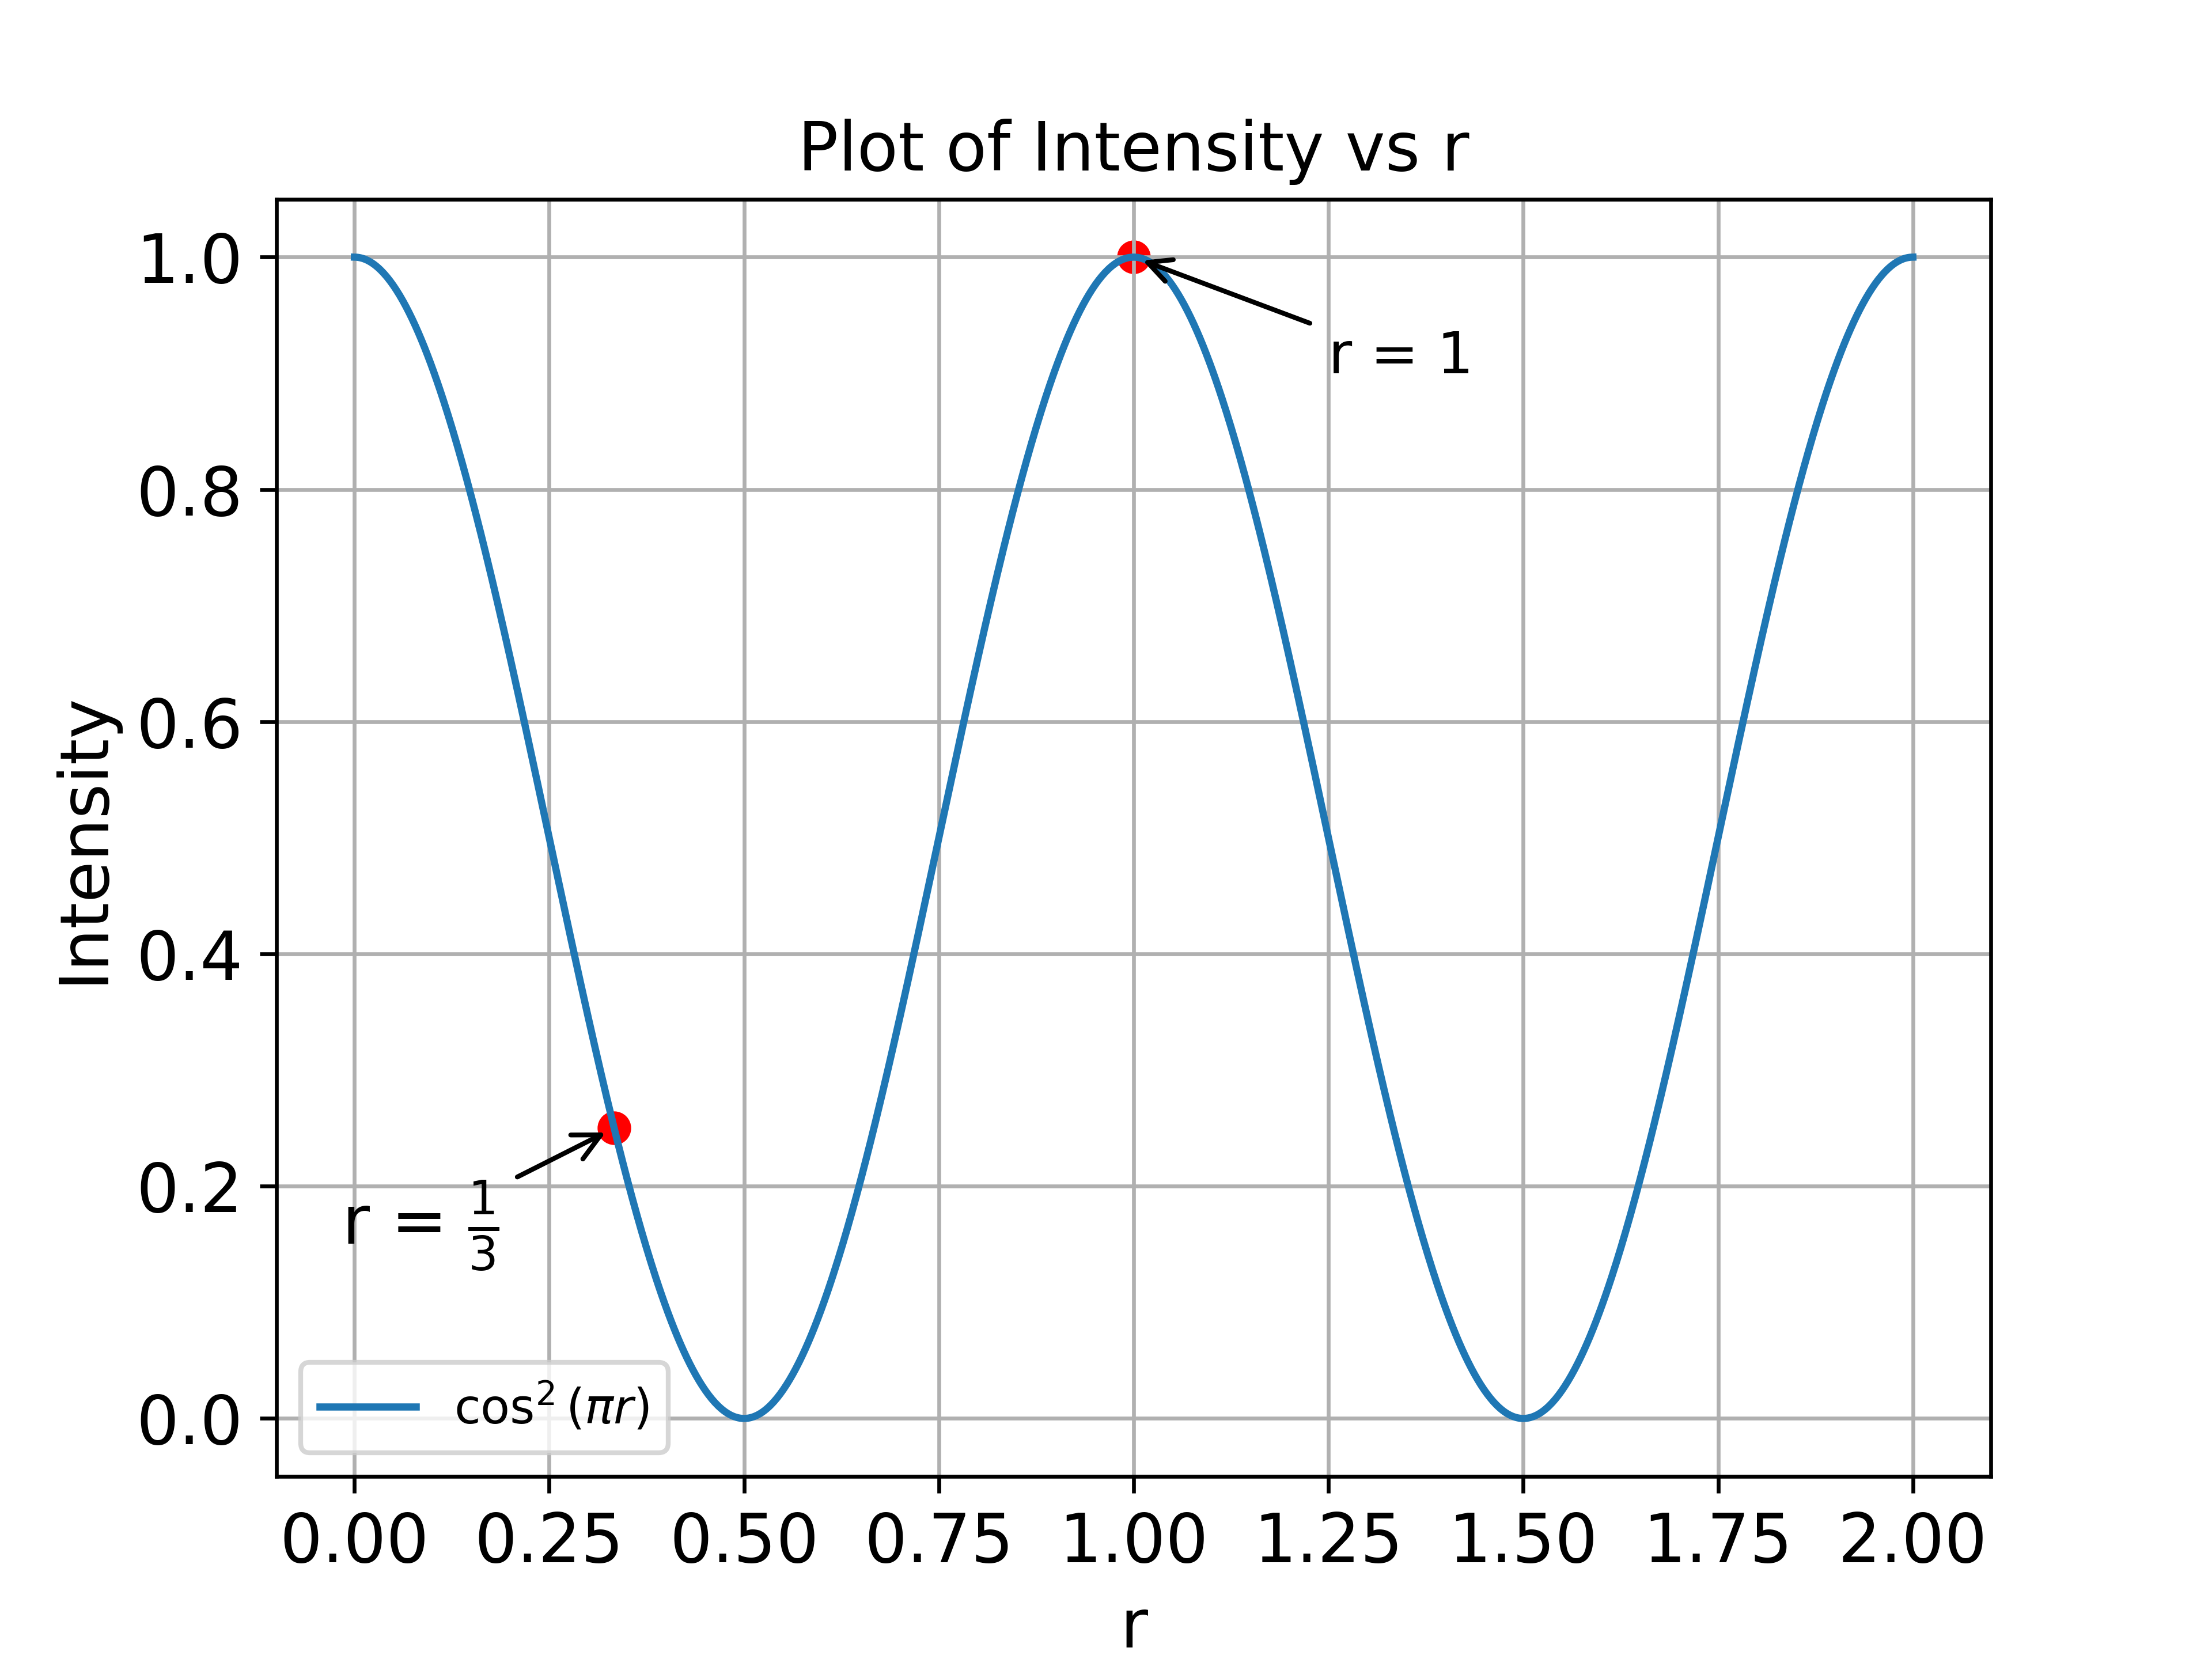
\includegraphics[width = \columnwidth]{figs/intensity_plot.png}
  \caption{}
    \label{fig:graph1}
\end{figure}
\bibliographystyle{IEEEtran}
\end{document}

\pagebreak

\item In a plane electromagnetic wave, the electric field oscillates sinusoidally at a frequency of $2.0 \text{ x } 10^{10}$ Hz and amplitude 48 $Vm^{-1}$.
\begin{enumerate}[label=(\alph*)]
    \item What is the wavelength of the wave?
    \item What is the amplitude of the oscillating magnetic field?
    \item Show that the average energy density of the $\vec{E}$ field equals the
average energy density of the $\vec{B}$ field. $[c = 3 \text{ x } 10^{8}ms^{-1} ]$
\end{enumerate}

\item \begin{enumerate}
\item For the wave on the string $y(x, t) = 0.06 \sin(\frac{2\pi x}{3}) \cos(120\pi t)$ , do all the points on the string     oscillate with the same (a)frequency , (b)phase , (c)amplitude ? Explain your answers. \\

 \item What is the amplitude of a point 0.375m away from one end? \\
 \end{enumerate}
 \solution
 \pagebreak
 
 \item 
 A transverse harmonic wave on a string is described by
\begin{align}
    y\brak{x,t}=3.0 \sin\brak{36t+0.018x+\frac{\pi}{4}}
\end{align}
where $x$ and $y$ are in cm and $t$ in s. The positive direction of $x$ is from left to right.
\begin{enumerate}[label=(\alph*)]
    \item Is this a travelling wave or a stationary wave? If it is travelling, what are the speed and direction of its propogation?
    \item What are its amplitude and frequency?
    \item What is the initial phase at the origin?
    \item  What is the least distance between two succesive crests in the wave?
\end{enumerate}

\solution
\pagebreak

\item In deriving the single slit diffraction pattern, it was stated that the intensity is zero at angles of $\frac{n\lambda}{a}$. Justify this by suitably dividing the slit to bring out the cancellation.\\
\solution
\pagebreak

\item A 60 $\mu$ F capacitor is connected to a 110 V, 60 Hz ac supply. Determine the rms value of the current in the circuit.\\
\solution
\pagebreak

\item A charged  $30\mu F$ capacitor is connected to a $27 mH$ inductor. What is the angular frequency of free oscillations of the circuit?\\
\solution
\pagebreak
\item Obtain the resonance frequency of a series LCR circuit with $L = 2.0\, H$, $C = 32\, \mu F$, and $R = 10\, \Omega$. What is the Q-value of the circuit.\\
\solution
\pagebreak
\item A charged 30 $\mu$F capacitor is connected to a 27 mH inductor. Suppose the initial charge on the capacitor is 6mC.What is the total energy stored in the circuit initially? What is the
total energy at later time? \\
\solution
\pagebreak

\item A wire stretched between two rigid supports vibrates in its fundamental mode with a frequency of $45 \, \text{Hz}$. The mass of the wire is $3.5 \times 10^{-2} \, \text{kg}$, and its linear mass density is $4.0 \times 10^{-2} \, \text{kg/m}$. The length of the wire is $0.875 \, \text{m}$. Determine the speed of a transverse wave on the string and the tension in the string.\\
\solution
\pagebreak

\item The given figure shows a series LCR circuit connected to a variable
frequency 230 V source. \\
L = 5.0 H, C = 80 $\mu$F, R = 40 $\Omega$.

\begin{figure}[h!]
\begin{center}
\begin{circuitikz}[american voltages]
      \draw (0,0)
      to[sV, l=$\varepsilon$] (0,2) 
      to[R, l=$R$, v=$V_R$] (4,2) 
      to[C, l=$C$, v=$V_C$] (4,0)
      to[L, l=$L$, v=$V_L$] (0,0);
\end{circuitikz}
\end{center}
\end{figure}

\begin{enumerate}
    \item Determine the source frequency which drives the circuit in resonance.
    \item Obtain the impedance of the circuit and the amplitude of current
at the resonating frequency.
    \item Determine the rms potential drops across the three elements of
the circuit. Show that the potential drop across the LC
combination is zero at the resonating frequency.\\
\end{enumerate}
\solution
\pagebreak

\item Q23) A narrow sound pulse (for example, a short pip by a whistle) is sent across a
	medium.\\ \brak{\text{a}} Does the pulse have a definite \brak{\text{i}} frequency, \brak{\text{ii}} wavelength, \brak{\text{iii}} speed
	of propagation?\\[1ex]\brak{\text{b}} If the pulse rate is 1 after every 20 s, (that is the whistle is
	blown for a split of second after every 20 s), Is the frequency of note produced
	by whistle equal to 1/20 or 0.05 Hz ?\\
\solution
\pagebreak
\item Suppose that the electric field part of an electromagnetic wave in vacuum given as\\ \textbf{E} =\{(3.1N/C)cos[(1.8 rad/m)y+(5.4$\times$10$^{6}$rad/s)t]\}$\vec{e_1}$ \\
(a) What is the direction of propagation ?\\
(b) What is the wavelength ? \\
(c) What is the frequency ?\\
(d) What is the amplitude of the magnetic field part of the wave?\\
(e) Write an expression for the magnetic field part of the wave.\\
\solution
 \iffalse
\let\negmedspace\undefined
\let\negthickspace\undefined
\documentclass[journal,12pt,twocolumn]{IEEEtran}
\usepackage{xparse}
\usepackage{cite}
\usepackage{amsmath,amssymb,amsfonts,amsthm}
\usepackage{algorithmic}
\usepackage{graphicx}
\usepackage{textcomp}
\usepackage{xcolor}
\usepackage{txfonts}
\usepackage{listings}
\usepackage{enumitem}
\usepackage{mathtools}
\usepackage{gensymb}
\usepackage{comment}
\usepackage[breaklinks=true]{hyperref}
\usepackage{tkz-euclide} 
\usepackage{listings}
\usepackage{gvv}                                        
\def\inputGnumericTable{}                                 
\usepackage[latin1]{inputenc}                                
\usepackage{color}                                            
\usepackage{array}                                            
\usepackage{longtable}                                       
\usepackage{calc}                                             
\usepackage{multirow}                                         
\usepackage{hhline}                                           
\usepackage{ifthen}                                           
\usepackage{lscape}

\newtheorem{theorem}{Theorem}[section]
\newtheorem{problem}{Problem}
\newtheorem{proposition}{Proposition}[section]
\newtheorem{lemma}{Lemma}[section]
\newtheorem{corollary}[theorem]{Corollary}
\newtheorem{example}{Example}[section]
\newtheorem{definition}[problem]{Definition}
\newcommand{\BEQA}{\begin{eqnarray}}
\newcommand{\EEQA}{\end{eqnarray}}
\newcommand{\define}{\stackrel{\triangle}{=}}
\theoremstyle{remark}
\newtheorem{rem}{Remark}
\begin{document}

\bibliographystyle{IEEEtran}
\vspace{3cm}

\title{ANALOG NCERT 12.8.11}
\author{EE23BTECH11046 - Poluri Hemanth$^{*}$}
\maketitle
\textbf{Question:}
Suppose that the electric field part of an electromagnetic wave
in vacuum given as\\ \textbf{E} =\{(3.1N/C)cos[(1.8 rad/m)y+(5.4$\times$10$^{6}$rad/s)t]\}$\vec{e_1}$ \\
(a) What is the direction of propagation ?\\
(b) What is the wavelength ? \\
(c) What is the frequency ?\\
(d) What is the amplitude of the magnetic field part of the wave?\\
(e) Write an expression for the magnetic field part of the wave.\\
\textbf{Solution:}
\fi
\begin{table}[h!]
    % Change address in github
    %%%%%%%%%%%%%%%%%%%%%%%%%%%%%%%%%%%%%%%%%%%%%%%%%%%%%%%%%%%%%%%%%%%%%%
%%                                                                  %%
%%  This is the header of a LaTeX2e file exported from Gnumeric.    %%
%%                                                                  %%
%%  This file can be compiled as it stands or included in another   %%
%%  LaTeX document. The table is based on the longtable package so  %%
%%  the longtable options (headers, footers...) can be set in the   %%
%%  preamble section below (see PRAMBLE).                           %%
%%                                                                  %%
%%  To include the file in another, the following two lines must be %%
%%  in the including file:                                          %%
%%        \def\inputGnumericTable{}                                 %%
%%  at the beginning of the file and:                               %%
%%        \input{name-of-this-file.tex}                             %%
%%  where the table is to be placed. Note also that the including   %%
%%  file must use the following packages for the table to be        %%
%%  rendered correctly:                                             %%
%%    \usepackage[latin1]{inputenc}                                 %%
%%    \usepackage{color}                                            %%
%%    \usepackage{array}                                            %%
%%    \usepackage{longtable}                                        %%
%%    \usepackage{calc}                                             %%
%%    \usepackage{multirow}                                         %%
%%    \usepackage{hhline}                                           %%
%%    \usepackage{ifthen}                                           %%
%%  optionally (for landscape tables embedded in another document): %%
%%    \usepackage{lscape}                                           %%
%%                                                                  %%
%%%%%%%%%%%%%%%%%%%%%%%%%%%%%%%%%%%%%%%%%%%%%%%%%%%%%%%%%%%%%%%%%%%%%%



%%  This section checks if we are begin input into another file or  %%
%%  the file will be compiled alone. First use a macro taken from   %%
%%  the TeXbook ex 7.7 (suggestion of Han-Wen Nienhuys).            %%
\def\ifundefined#1{\expandafter\ifx\csname#1\endcsname\relax}


%%  Check for the \def token for inputed files. If it is not        %%
%%  defined, the file will be processed as a standalone and the     %%
%%  preamble will be used.                                          %%
\ifundefined{inputGnumericTable}

%%  We must be able to close or not the document at the end.        %%
	\def\gnumericTableEnd{\end{document}}


%%%%%%%%%%%%%%%%%%%%%%%%%%%%%%%%%%%%%%%%%%%%%%%%%%%%%%%%%%%%%%%%%%%%%%
%%                                                                  %%
%%  This is the PREAMBLE. Change these values to get the right      %%
%%  paper size and other niceties.                                  %%
%%                                                                  %%
%%%%%%%%%%%%%%%%%%%%%%%%%%%%%%%%%%%%%%%%%%%%%%%%%%%%%%%%%%%%%%%%%%%%%%

	\documentclass[12pt%
			  %,landscape%
                    ]{report}
       \usepackage[latin1]{inputenc}
       \usepackage{fullpage}
       \usepackage{color}
       \usepackage{array}
       \usepackage{longtable}
       \usepackage{calc}
       \usepackage{multirow}
       \usepackage{hhline}
       \usepackage{ifthen}

	\begin{document}


%%  End of the preamble for the standalone. The next section is for %%
%%  documents which are included into other LaTeX2e files.          %%
\else

%%  We are not a stand alone document. For a regular table, we will %%
%%  have no preamble and only define the closing to mean nothing.   %%
    \def\gnumericTableEnd{}

%%  If we want landscape mode in an embedded document, comment out  %%
%%  the line above and uncomment the two below. The table will      %%
%%  begin on a new page and run in landscape mode.                  %%
%       \def\gnumericTableEnd{\end{landscape}}
%       \begin{landscape}


%%  End f the else clause for this file being \input.              %%
\fi

%%%%%%%%%%%%%%%%%%%%%%%%%%%%%%%%%%%%%%%%%%%%%%%%%%%%%%%%%%%%%%%%%%%%%%
%%                                                                  %%
%%  The rest is the gnumeric table, except for the closing          %%
%%  statement. Changes below will alter the table's appearance.     %%
%%                                                                  %%
%%%%%%%%%%%%%%%%%%%%%%%%%%%%%%%%%%%%%%%%%%%%%%%%%%%%%%%%%%%%%%%%%%%%%%

\providecommand{\gnumericmathit}[1]{#1} 
%%  Uncomment the next line if you would like your numbers to be in %%
%%  italics if they are italizised in the gnumeric table.           %%
%\renewcommand{\gnumericmathit}[1]{\mathit{#1}}
\providecommand{\gnumericPB}[1]%
{\let\gnumericTemp=\\#1\let\\=\gnumericTemp\hspace{0pt}}
 \ifundefined{gnumericTableWidthDefined}
        \newlength{\gnumericTableWidth}
        \newlength{\gnumericTableWidthComplete}
        \newlength{\gnumericMultiRowLength}
        \global\def\gnumericTableWidthDefined{}
 \fi
%% The following setting protects this code from babel shorthands.  %%
 \ifthenelse{\isundefined{\languageshorthands}}{}{\languageshorthands{english}}
%%  The default table format retains the relative column widths of  %%
%%  gnumeric. They can easily be changed to c, r or l. In that case %%
%%  you may want to comment out the next line and uncomment the one %%
%%  thereafter                                                      %%
\providecommand\gnumbox{\makebox[0pt]}
%%\providecommand\gnumbox[1][]{\makebox}

%% to adjust positions in multirow situations                       %%
\setlength{\bigstrutjot}{\jot}
\setlength{\extrarowheight}{\doublerulesep}

%%  The \setlongtables command keeps column widths the same across  %%
%%  pages. Simply comment out next line for varying column widths.  %%
\setlongtables

\setlength\gnumericTableWidth{%
	30pt+%
	60pt+%
	185pt+%
0pt}
\def\gumericNumCols{3}
\setlength\gnumericTableWidthComplete{\gnumericTableWidth+%
         \tabcolsep*\gumericNumCols*2+\arrayrulewidth*\gumericNumCols}
\ifthenelse{\lengthtest{\gnumericTableWidthComplete > \linewidth}}%
         {\def\gnumericScale{1*\ratio{\linewidth-%
                        \tabcolsep*\gumericNumCols*2-%
                        \arrayrulewidth*\gumericNumCols}%
{\gnumericTableWidth}}}%
{\def\gnumericScale{1}}

%%%%%%%%%%%%%%%%%%%%%%%%%%%%%%%%%%%%%%%%%%%%%%%%%%%%%%%%%%%%%%%%%%%%%%
%%                                                                  %%
%% The following are the widths of the various columns. We are      %%
%% defining them here because then they are easier to change.       %%
%% Depending on the cell formats we may use them more than once.    %%
%%                                                                  %%
%%%%%%%%%%%%%%%%%%%%%%%%%%%%%%%%%%%%%%%%%%%%%%%%%%%%%%%%%%%%%%%%%%%%%%

\ifthenelse{\isundefined{\gnumericColA}}{\newlength{\gnumericColA}}{}\settowidth{\gnumericColA}{\begin{tabular}{@{}p{30pt*\gnumericScale}@{}}x\end{tabular}}
\ifthenelse{\isundefined{\gnumericColB}}{\newlength{\gnumericColB}}{}\settowidth{\gnumericColB}{\begin{tabular}{@{}p{60pt*\gnumericScale}@{}}x\end{tabular}}
\ifthenelse{\isundefined{\gnumericColC}}{\newlength{\gnumericColC}}{}\settowidth{\gnumericColC}{\begin{tabular}{@{}p{185pt*\gnumericScale}@{}}x\end{tabular}}

\begin{tabular}[c]{%
	b{\gnumericColA}%
	b{\gnumericColB}%
	b{\gnumericColC}%
	}

%%%%%%%%%%%%%%%%%%%%%%%%%%%%%%%%%%%%%%%%%%%%%%%%%%%%%%%%%%%%%%%%%%%%%%
%%  The longtable options. (Caption, headers... see Goosens, p.124) %%
%	\caption{The Table Caption.}             \\	%
% \hline	% Across the top of the table.
%%  The rest of these options are table rows which are placed on    %%
%%  the first, last or every page. Use \multicolumn if you want.    %%

%%  Header for the first page.                                      %%
%	\multicolumn{3}{c}{The First Header} \\ \hline 
%	\multicolumn{1}{c}{colTag}	%Column 1
%	&\multicolumn{1}{c}{colTag}	%Column 2
%	&\multicolumn{1}{c}{colTag}	\\ \hline %Last column
%	\endfirsthead

%%  The running header definition.                                  %%
%	\hline
%	\multicolumn{3}{l}{\ldots\small\slshape continued} \\ \hline
%	\multicolumn{1}{c}{colTag}	%Column 1
%	&\multicolumn{1}{c}{colTag}	%Column 2
%	&\multicolumn{1}{c}{colTag}	\\ \hline %Last column
%	\endhead

%%  The running footer definition.                                  %%
%	\hline
%	\multicolumn{3}{r}{\small\slshape continued\ldots} \\
%	\endfoot

%%  The ending footer definition.                                   %%
%	\multicolumn{3}{c}{That's all folks} \\ \hline 
%	\endlastfoot
%%%%%%%%%%%%%%%%%%%%%%%%%%%%%%%%%%%%%%%%%%%%%%%%%%%%%%%%%%%%%%%%%%%%%%

\hhline{|-|-|-}
	\multicolumn{1}{|p{\gnumericColA}|}%
	{\gnumericPB{\centering}\gnumbox{\textbf{Symbol}}}
	&\multicolumn{1}{p{\gnumericColB}|}%
	{\gnumericPB{\centering}\gnumbox{\textbf{Values}}}
	&\multicolumn{1}{p{\gnumericColC}|}%
	{\gnumericPB{\centering}\gnumbox{\textbf{Description}}}

	
\\
\hhline{|---|}
	\multicolumn{1}{|p{\gnumericColA}|}%
	{\gnumericPB{\centering}\gnumbox{$\lambda$}}
	&\multicolumn{1}{p{\gnumericColB}|}%
	{\gnumericPB{\centering}\gnumbox{$\frac{2\pi}{k}$}}
	&\multicolumn{1}{p{\gnumericColC}|}%
	{\gnumericPB{\centering}\gnumbox{Wave length of E.M wave.}}



\\
\hhline{|---|}
	\multicolumn{1}{|p{\gnumericColA}|}%
	{\gnumericPB{\centering}\gnumbox{$f$}}
	&\multicolumn{1}{p{\gnumericColB}|}%
	{\gnumericPB{\centering}\gnumbox{$0.859\times10^{6}Hz$}}
	&\multicolumn{1}{p{\gnumericColC}|}%
	{\gnumericPB{\centering}\gnumbox{Frequency of E.M wave.}}


\\
\hhline{|---|}
	\multicolumn{1}{|p{\gnumericColA}|}%
	{\gnumericPB{\centering}\gnumbox{$c$}}             
        &\multicolumn{1}{p{\gnumericColB}|}%
	{\gnumericPB{\centering}\gnumbox{$3\times10^{6}m/s$}}  
        &\multicolumn{1}{p{\gnumericColC}|}%
	{\gnumericPB{\centering}\gnumbox{Velocity of propagation of E.M wave.}}

\\
\hhline{|---|}
	\multicolumn{1}{|p{\gnumericColA}|}%
	{\gnumericPB{\centering}\gnumbox{$\omega$}}             
        &\multicolumn{1}{p{\gnumericColB}|}%
        {\gnumericPB{\centering}\gnumbox{$2\pi f$}}  
        &\multicolumn{1}{p{\gnumericColC}|}%
	{\gnumericPB{\centering}\gnumbox{Angular frequency of E.M wave.}}

\\
\hhline{|---|}
	\multicolumn{1}{|p{\gnumericColA}|}%
        {\gnumericPB{\centering}\gnumbox{$k$}}        
        &\multicolumn{1}{p{\gnumericColB}|}%
        {\gnumericPB{\centering}\gnumbox{$1.8 rad/m$}}
        &\multicolumn{1}{p{\gnumericColC}|}%
        {\gnumericPB{\centering}\gnumbox{Wave number of E.M wave}}   
\\
\hhline{|---|}
        \multicolumn{1}{|p{\gnumericColA}|}%
        {\gnumericPB{\centering}\gnumbox{$B_o$}}        
        &\multicolumn{1}{p{\gnumericColB}|}%
	{\gnumericPB{\centering}\gnumbox{$\frac{E_o}{c}$}}
        &\multicolumn{1}{p{\gnumericColC}|}%
        {\gnumericPB{\centering}\gnumbox{Amplitude of magnetic part of E.M wave }}   
\\
\hhline{|---|}
        \multicolumn{1}{|p{\gnumericColA}|}%
        {\gnumericPB{\centering}\gnumbox{$E_o$}}        
        &\multicolumn{1}{p{\gnumericColB}|}%
        {\gnumericPB{\centering}\gnumbox{$3.1N/C$}}
        &\multicolumn{1}{p{\gnumericColC}|}%
        {\gnumericPB{\centering}\gnumbox{Amplitude of electric part of E.M wave.}}   
\\
\hhline{|---|}
        \multicolumn{1}{|p{\gnumericColA}|}%
	{\gnumericPB{\centering}\gnumbox{$\vec{e_1}$}}        
        &\multicolumn{1}{p{\gnumericColB}|}%
        {\gnumericPB{\centering}\gnumbox{-}}
        &\multicolumn{1}{p{\gnumericColC}|}%
        {\gnumericPB{\centering}\gnumbox{Base vector in direction of electric field.}} 	
\\
\hhline{|---|}
        \multicolumn{1}{|p{\gnumericColA}|}%
	{\gnumericPB{\centering}\gnumbox{$\vec{e_2}$}}        
        &\multicolumn{1}{p{\gnumericColB}|}%
        {\gnumericPB{\centering}\gnumbox{-}}
        &\multicolumn{1}{p{\gnumericColC}|}%
        {\gnumericPB{\centering}\gnumbox{Base vector in direction of propagation.}} 
\\
\hhline{|---|}
        \multicolumn{1}{|p{\gnumericColA}|}%
	{\gnumericPB{\centering}\gnumbox{$\vec{e_3}$}}        
        &\multicolumn{1}{p{\gnumericColB}|}%
        {\gnumericPB{\centering}\gnumbox{-}}
        &\multicolumn{1}{p{\gnumericColC}|}%
        {\gnumericPB{\centering}\gnumbox{Base vector in direction of magnetic field.}} 
\\
\hhline{|-|-|-|}
\end{tabular}

\ifthenelse{\isundefined{\languageshorthands}}{}{\languageshorthands{\languagename}}
\gnumericTableEnd

    \caption{Input Parameters}
    \label{tab:12.8.11}
\end{table}\\
(a)\\
As the wave is in form of $cos(ky+wt)$
the wave is propagating along $-y$ axis, represented by $\vec{e_2}$\\
(b)
\begin{align}
	k&=\frac{2\pi}{\lambda} \\
	\Rightarrow\lambda&=\frac{2\pi}{1.8}\\
	&\approx3.5m
\end{align}
(c)
\begin{align} 
	\omega&=2\pi.f \\
	 5.4 x 10^{6} &=2.\pi.f \\
	\Rightarrow f &= 0.859 \times 10^{6} Hz    
\end{align}
(d)
\begin{align}
	B_o&=\frac{E_o}{c}
\end{align}
where $c$ is velocity of propagation of wave which is given by
\begin{align}
	c&=\frac{\omega}{k} \\
	&=\frac{5.4 \times 10^{6}}{1.8}\\
	&=3 \times 10^{6}m/s.\\
	B_o&= \frac{3.1}{3 \times 10^{6}}\\
	&= 1.03 \times 10^{-6}T\label{1}
\end{align}
(e)
Direction of magnetic field is $\vec{e_3}$\\
where,
\begin{align}
	\vec{e_3}&=\vec{e_2} \times \vec{e_1}\\
	\textbf{B}&=B_ocos(ky+wt)\vec{e_3}\label{b}
\end{align}
 From \eqref{1},\eqref{b}
\begin{align}
	\textbf{B}=1.03\times10^{-6}T\{cos[(1.8rad/m)y+(5.4x10^{6}rad/s)t]\}\vec{e_3}
\end{align}
\begin{figure}[h]
\centering
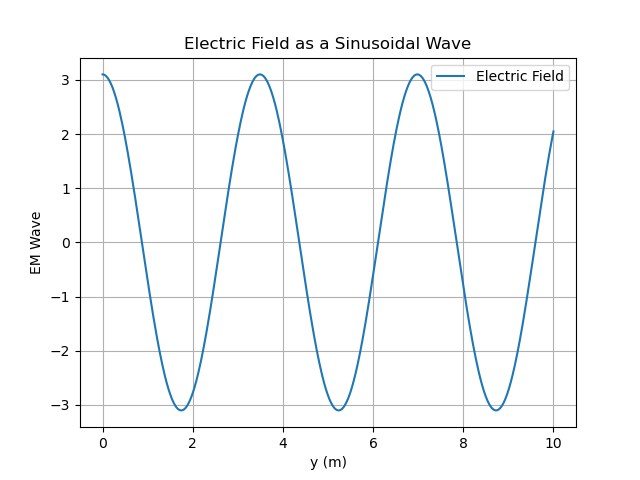
\includegraphics[width=1\columnwidth]{ncert-physics/12/8/11/figures/ewave.png}
\caption{Electric field part}
\label{solution}
\end{figure}
\begin{figure}[h]
\centering
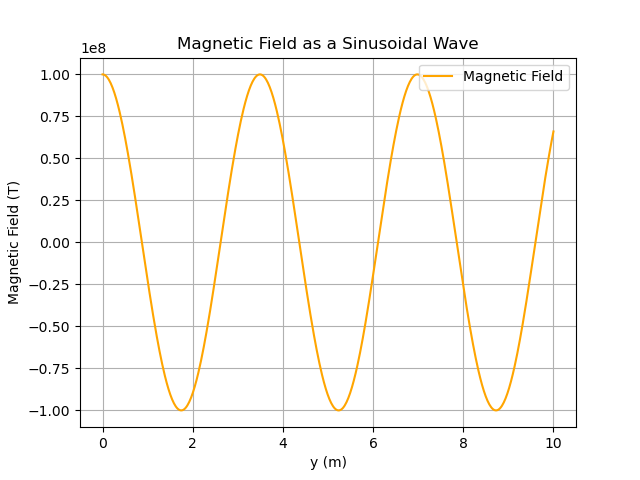
\includegraphics[width=1\columnwidth]{ncert-physics/12/8/11/figures/mwave.png}
\caption{Magnetic field part}
\label{solution}
\end{figure}



%\end{document}


\pagebreak

\item A 44 mH inductor is connected to 220 V, 50 Hz ac supply. Determine
the rms value of the current in the circuit.\\
\solution
\iffalse
\documentclass[journal,12pt,twocolumn]{IEEEtran}
\usepackage{amsmath,amssymb,amsfonts,amsthm}
\usepackage{txfonts}
\usepackage{tkz-euclide}
\usepackage{listings}
\usepackage{gvv}
\usepackage[latin1]{inputenc}
\usepackage{adjustbox}
\usepackage{array}
\usepackage{tabularx}
\usepackage{pgf}
\usepackage{lmodern}
\usepackage{circuitikz}
\usepackage{tikz}
\usepackage{graphicx}
\begin{document}
\bibliographystyle{IEEEtran}

\vspace{3cm}

\title{}
\author{EE23BTECH11047 - Deepakreddy P
}
\maketitle
\newpage
\bigskip


\noindent \textbf{3} \quad A 44 mH inductor is connected to 220 V, 50 Hz ac supply. Determine
the rms value of the current in the circuit.\\
\solution
\fi


\begin{figure}[ht]
  \centering
      \begin{circuitikz}[american]
   \draw (0,0) to [L=44mH](0,3) to (3,3)[short] to [sV=220V](3,0) to [short](0,0);
\end{circuitikz}

  \caption{Circuit-1}
\end{figure}

\begin{align}
    V &= I \brak{j \omega L} \\
    I &= \frac{V}{j \omega L} A \\
    I &= \frac{220 \sqrt{2}}{j \brak{314} \brak{44 \text{x} 10^{-3}}}A\\
    I &= \frac{22.52}{j}A
\end{align}


\begin{figure}[ht]
  \centering

      \begin{circuitikz}[american]
   \draw (0,0) to [L=$44j\omega $](0,3) to (3,3)[short] to [sV=220V](3,0) to [short](0,0);
\end{circuitikz}


  \caption{Circuit-2}
\end{figure}

\begin{align}
    I_{rms} = \frac{I}{\sqrt{2}}A\\
    I_{rms} = \frac{15.92}{j}A\\
    \abs{I_{rms}} = 15.92 A
\end{align}

\begin{figure}[ht]
   \centering
   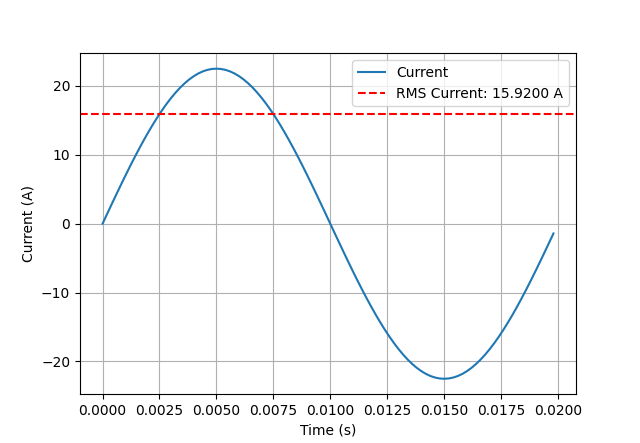
\includegraphics[width=1.1\columnwidth]{ncert-physics/12/7/3/figs/ac.png}
   \caption{Plot of I vs time}
\end{figure}

\begin{center}
    \begin{table}[ht]
        \setlength{\arrayrulewidth}{0.3mm}
\setlength{\tabcolsep}{12pt}
\renewcommand{\arraystretch}{1.3}


\begin{center}
\caption{Input Parameters}
\begin{tabular}{ |p{1.7cm}|p{1.7cm}|p{1.7cm}|  }

\hline
 {Symbol}&{Description} & {value}\\
\hline
L & Inductor & 44mH\\
\hline
$V_{rms}$ & RMS Voltage  & 220V\\
\hline
f & Frequency & 50Hz \\
\hline

\end{tabular}
\end{center}

    \end{table}
\end{center}

\begin{center}
    \begin{table}[ht]
        \setlength{\arrayrulewidth}{0.3mm}
\setlength{\tabcolsep}{12pt}
\renewcommand{\arraystretch}{1.3}


\begin{center}
\caption{Formulae and output}
\begin{tabular}{ |p{1.5cm}|p{1.5cm}|p{1.5cm}|p{1.5cm}|  }

\hline
{Symbol} & {Description} & {Formulae} & {Value} \\
\hline
$X_{L}$ & Inductive Reactance & 2 $\pi fL$ & 13.816 $\Omega$ \\
\hline
$\omega$ & Angular Frequency & $2\pi f$ & 314 rad/sec \\
\hline
$I_{rms}$ & Rms current & $\frac{V}{X_{L}}$ & 15.92A \\
\hline


\end{tabular}
\end{center}

    \end{table}
\end{center}

%\end{document}


\pagebreak

\item The 6563 \AA\, H$\alpha$ line emitted by hydrogen in a star is found to be redshifted by 15 \AA. Estimate the speed with which the star is receding from the Earth.
\solution
\pagebreak
\item The amplitude  of the magnetic part of a harmonic elctromagnetic wave is $B_0=510$nT.What is the amplitude of the electric part of the electromagnetic wave.\\
\solution
\pagebreak

\item A 100$\mu$F capacitor in series with a 40$\Omega$ resistance is connected to a 110V, 60Hz supply.
\begin{enumerate}[label = {\brak{\alph*}}]
\item What is the maximum current in the circuit?
\item What is the time lag between the current maximum and the voltage maximum?\\
\end{enumerate}
\solution
\pagebreak
\item A 100 $\ohm$ resistor is connected to $220 V$, $50 Hz$ AC supply.\\
(1) What is the rms value of current in the circuit?\\
(2) What is the net power consumed over a full cycle?

\solution
\pagebreak
\item  Two towers on top of two hills are $40$ km apart.This line joining them passes $50$ m above a hill halfway between the towers.What is the longest wavelength of radio waves,which can be sent between the towers without  appereciable diffraction effects?\\
\solution
\pagebreak
\item A circuit containing a 80mH inductor and a 60$\mu$F capacitor in series is connected to a 230V, 50Hz supply. The resistance of the circuit is negligible.\\
\begin{enumerate}
  \item Obtain the current amplitude and rms value.
  \item Obtain the rms value of potential drops across each element.
  \item What is the average power transferred to the inductor ?
  \item What is the average power transferred to the capacitor ?
  \item What is the total average power absorbed by the circuit ? \brak{\text{'Average' implies 'averaged over one cycle'.}}
\end{enumerate}
\solution
\pagebreak
\item A coil of inductance 0.50 H and resistance 100 $\Omega$ is connected to a 240 V, 50 Hz ac supply.\\
(a) What is the maximum current in the coil?\\		
(b) What is the time lag between the voltage maximum and the current maximum?\\
\solution
\pagebreak

\item A plane electromagnetic wave travels in vacuum along the \(z\)-direction. What can you say about the directions of its electric (\(\mathbf{E}\)) and magnetic (\(\mathbf{B}\)) field vectors? If the frequency of the wave is \(30 \, \text{MHz}\), what can you say about its wavelength?\\
\solution
\pagebreak

\item
Earthquakes generate sound waves inside the earth. Unlike a gas, the earth can experience both transverse (S) and longitudinal (P) sound waves. Typically the speed of S wave is about $4.0 km/s$, and that of P wave is $8.0 km/s$. A seismograph records P and S waves from an earthquake. The first P wave arrives $4 min$ before the first S wave. Assuming the waves travel in straight line, at what distance does the
earthquake occur ?
\solution
\pagebreak

\item
A hospital uses an ultrasonic scanner to locate tumors in a tissue. What is the wavelength of sound in the tissue in which the speed of sound is $1.7 \, \text{km/s}$? The operating frequency of the scanner is $4.2 \, \text{MHz}$.
\solution
\pagebreak

\item In double-slit experiment using light of wavelength $600 nm$, the
angular width of a fringe formed on a distant screen is $0.1\degree$. What is
the spacing between the two slits?\\
\solution
\pagebreak

\item A spring having with a spring constant 1200 N$m^{-1}$ is mounted on a horizontal
table as shown in Fig.A mass of 3 kg is attached to the free end of the
spring. The mass is then pulled sideways to a distance of 2.0 cm and released.\\
Determine (i) the frequency of oscillations, (ii) maximum acceleration of the mass,
and (iii) the maximum speed of the mass.
\begin{figure}[h!]
    \centering
    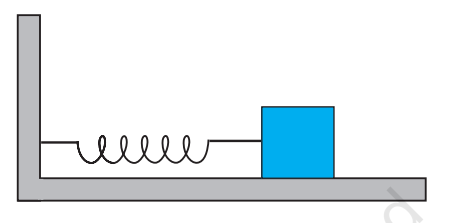
\includegraphics[width=0.5\linewidth]{ncert-physics/11/14/9/figs/analog.png}
    \caption{ }

\end{figure}
\solution
\pagebreak


\item A string of mass 2.50 kg is under a tension of 200 N. The length of the stretched string is 20.0 m. If the transverse jerk is struck at one end of the string, how long does he disturbance take to reach the other end ? 
\solution
\pagebreak

\item In a Young's double-slit experiment, the slits ar e separated by $0.28$ mm and the screen is placed $1.4 m$ away. The distance between the central bright fringe and the fourth bright fringe is measured to be $1.2 cm$. Determine the wavelength of light used in the experiment.\\
\solution
\pagebreak
\item Keeping the source frequency equal to the resonating frequency of the series $LCR$ circuit, if the three elements, $L, C$, and $R$ are arranged in parallel, show that the total current in the parallel $LCR$ circuit is minimum at this frequency. Obtain the current rms value in each branch of the circuit for the elements and source specified in Exercise 7.11 for this frequency\\
   $\varepsilon =230V$, $L=5.0H$, $C=80\mu$F, $R=40\ohm$\\
\begin{circuitikz}
  \draw (0,0) to[sV, v=$\varepsilon$] (0,3);
  \draw (0,3) to [resistor, l=$R$] (3,3);
  \draw (3,3)to[capacitor,l=$C$] (3,0);
  \draw (0,0)to[L,l=$L$] (3,0);
\end{circuitikz}
\\ \\ \\
\begin{circuitikz}
    \draw (0,0) to [sV, v=$\varepsilon$] (0,3);
    \draw (2,3) to [R, l=$R$] (2,0);
    \draw (4,3) to [C, l=$C$] (4,0);
    \draw (6,3) to [L, l=$L$] (6,0);
    \draw (0,0) -- (6,0);
    \draw (0,3) -- (6,3);
\end{circuitikz}
 \solution
\item A SONAR system fixed in a submarine operates at a frequency 40.0 kHz. An enemy submarine moves towards the SONAR with a speed of 360 km/hr. What is the frequency of sound reflected by the submarine? Take the speed of sound in water to be 1450 m/s.\\
\solution
\pagebreak

\item Figure 1.0.35 (a) shows a spring of force constant k clamped rigidly at one end and a mass $m$ attached to its free end. A force $F$ applied at the free end stretches the spring. Figure 1.0.35 (b) shows the same spring with both ends free and attached to a mass $m$ at either end. Each end of the spring in Fig. 1.0.35(b) is stretched by the same force $F$.

\begin{figure}[ht]
\caption{ }
    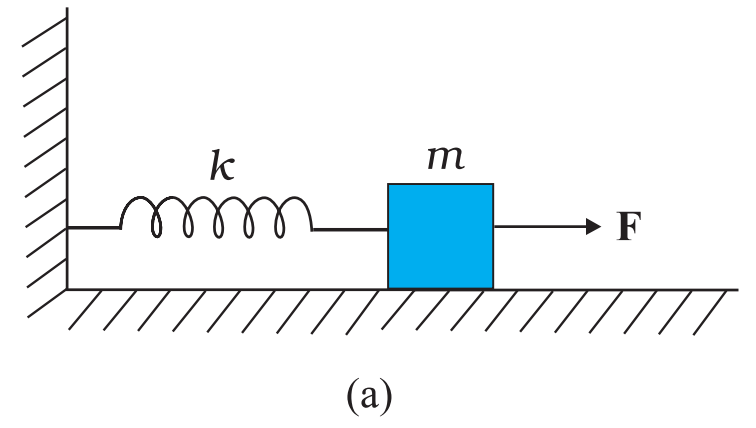
\includegraphics[width=0.45\textwidth]{ncert-physics/11/14/13/figs/fig1.png}
    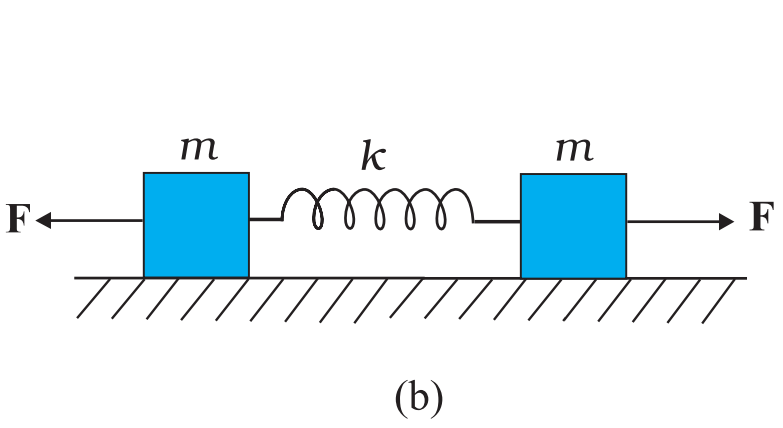
\includegraphics[width=0.45\textwidth]{ncert-physics/11/14/13/figs/fig2.png}
\end{figure}
\begin{enumerate}[label = (\alph*)]
  \item What is the maximum extension of the spring in the two cases ?    
  \item If the mass in Fig. (a) and the two masses in Fig. (b) are released, what is the
period of oscillation in each case ?
\end{enumerate}
    
\solution
\newpage

\item A bat is flitting about in a cave, navigating via ultrasonic beeps. Assume that the
sound emission frequency of the bat is 40 kHz. During one fast swoop directly
toward a flat wall surface, the bat is moving at 0.03 times the speed of sound in air.
What frequency does the bat hear reflected off the wall ? \hfill{NCERT Analog 11.15.27}\\
\solution
\pagebreak
\item One end of a long string of linear mass density $8.0 \times 10^{-3} \, \text{kg m}^{-1}$ is connected to an electrically driven tuning fork of frequency $256 \, \text{Hz}$. The other end passes over a pulley and is tied to a pan containing a mass of $90 \, \text{kg}$. The pulley end absorbs all the incoming energy so that reflected waves at this end have negligible amplitude. At $t=0$, the left end (fork end) of the string $x=0$ has zero transverse displacement ($y=0$) and is moving along positive $y$-direction. The amplitude of the wave is $5.0 \, \text{cm}$. Write down the transverse displacement $y$ as a function of $x$ and $t$ that describes the wave on the string.\hfill{NCERT Analog 11.15.24} \\
\solution
\pagebreak
\item A steel wire has a length of 12.0 m and a mass of 2.10 kg. What should be the
tension in the wire so that speed of a transverse wave on the wire equals the speed
of sound in dry air at 20 $^{\circ} C = 343ms^{-1}$ \hfill{NCERT Analog 11.15.3}\\
\solution
\pagebreak
\item What is the Brewster angle for air to glass transition?\brak{{\text{Refractive index of glass =1.5}}}\\
\solution
\pagebreak
\item A parallel beam of light with a wavelength of $500$ nm falls on a narrow slit, and the resulting diffraction pattern is observed on a screen $1$ m away. The distance to the first minimum from the center of the screen is $2.5$ mm.\\
Find the width of the slit given that $y = 0.0025$ m, $L = 1$ m, and $\lambda = 5 \times 10^{-7}$ m.\\
\solution
\pagebreak

\item Two sitar strings A and B playing the note `Ga' are slightly out of tune and produce beats of frequency $6$Hz. The tension in the string A is slightly reduced and the beat frequency is found to reduce to $3$Hz. If the original frequency of A is $324$Hz,what is the frequency of B?\\
\solution
\pagebreak

\item Which of the following functions of time represent (a) simple harmonic, (b) periodic
 but not simple harmonic, and (c) non-periodic motion? Give period for each case of periodic motion ($\omega$ is any positive constant):\\
 \begin{enumerate}
 \item $\sin\brak{\omega t}-\cos\brak{\omega t}$\\
 \item $\sin^3\brak{\omega t}$\\
 \item $3\cos\brak{\frac{\pi}{4}- 2\omega t}$\\
 \item $\cos\brak{\omega t}+\cos\brak{3\omega t}+\cos\brak{5\omega t}$\\
 \item \text{exp}\brak{-\omega^2 t^2}\\
 \item $1+\omega t+\omega^2 t^2$\\
  \end{enumerate}
 \solution
\iffalse
\let\negmedspace\undefined
\let\negthickspace\undefined
\documentclass[journal,12pt,onecolumn]{IEEEtran}
\usepackage{cite}
\usepackage{amsmath,amssymb,amsfonts,amsthm}
\usepackage{algorithmic}
\usepackage{graphicx}
\usepackage{textcomp}
\usepackage{xcolor}
\usepackage{txfonts}
\usepackage{listings}
\usepackage{enumitem}
\usepackage{mathtools}
\usepackage{gensymb}
\usepackage{comment}
\usepackage[breaklinks=true]{hyperref}
\usepackage{tkz-euclide} 
\usepackage{listings}
\usepackage{gvv}                                        
\def\inputGnumericTable{}                                 
\usepackage[latin1]{inputenc}                                
\usepackage{color}                                            
\usepackage{array}                                            
\usepackage{longtable}                                       
\usepackage{calc}                                             
\usepackage{multirow}                                         
\usepackage{hhline}                                           
\usepackage{ifthen}                                           
\usepackage{lscape}

\newtheorem{theorem}{Theorem}[section]
\newtheorem{problem}{Problem}
\newtheorem{proposition}{Proposition}[section]
\newtheorem{lemma}{Lemma}[section]
\newtheorem{corollary}[theorem]{Corollary}
\newtheorem{example}{Example}[section]
\newtheorem{definition}[problem]{Definition}
\newcommand{\BEQA}{\begin{eqnarray}}
 \newcommand{\EEQA}{\end{eqnarray}}
\newcommand{\define}{\stackrel{\triangle}{=}}
\theoremstyle{remark}
\newtheorem{rem}{Remark}
\begin{document}
 \bibliographystyle{IEEEtran}
 \vspace{3cm}
 \title{\textbf{11.14-4}}
 \author{EE23BTECH11048-Ponugumati Venkata Chanakya$^{*}$% <-this % stops a space
 }
 \maketitle

 \bigskip
 \renewcommand{\thefigure}{\theenumi}
 \renewcommand{\thetable}{\theenumi}
 \textbf{QUESTION:}
 Which of the following functions of time represent (a) simple harmonic, (b) periodic
 but not simple harmonic, and (c) non-periodic motion? Give period for each case of periodic motion ($\omega$ is any positive constant):\\
 \begin{enumerate}
 \item $\sin\brak{\omega t}-\cos\brak{\omega t}$\\
 \item $\sin^3\brak{\omega t}$\\
 \item $3\cos\brak{\frac{\pi}{4}- 2\omega t}$\\
 \item $\cos\brak{\omega t}+\cos\brak{3\omega t}+\cos\brak{5\omega t}$\\
 \item \text{exp}\brak{-\omega^2 t^2}\\
 \item $1+\omega t+\omega^2 t^2$\\
  \end{enumerate}
 \solution:\\
\fi
 \begin{enumerate}
   \item Periodic function:
   \begin{align}
x(t+T) = x(t) \quad \forall x \in \mathbb{R}
\end{align}
 where min $T$ s.t $T>0$ is time period\\
 \\
   \item SHM:\\
    For a function to be in shm it must satisfy 
    \begin{align}
   \frac{d^2 x(t)}{dt^2} = - (2\pi f_0)^2 x(t)
      \end{align}
      \end{enumerate}
   \begin{enumerate}
   \begin{table}[!ht]
    \centering
        
      \begin{tabular}{|c|c|c|} 
      \hline
\textbf{Variable}& \textbf{Description}& formula\\\hline
         $x(t)$&  Displacemen wrt mean position&none\\\hline
          $\omega$&Angular frequncy&$2\pi f$\\\hline
          $T$& Time period &$\frac{1}{f}$ \\ \hline
          $\phi$& phase angle &none \\ \hline
    \end{tabular}

    \caption{input parameters}
    \label{tab:}
\end{table}
\item $\sin(2\pi f t)- \cos(2\pi f t)$\\
The function can be rewritten as:
 \begin{align}
  &= \sin(2\pi f t) - \sin\brak{\frac{\pi}{2} - 2\pi f t}\\
  &=2 \cos\brak{\frac{\pi}{4}} \sin\brak{2\pi f t - \frac{\pi}{4}}\\
  &=\sqrt{2}\sin\brak{2\pi f t - \frac{\pi}{4}}\\
  \frac{d^2(\sin(2\pi f t)- \cos(2\pi f t))}{dt^2}&=-(2\pi f)^2(\sin(2\pi f t)- \cos(2\pi f t))\\
     \frac{d^2 x(t)}{dt^2} &= - (2\pi f)^2 x(t)\\
     \end{align}
     
 $\therefore$ SHM, $T$ is $\frac{1}{f}$and $\phi$ is $\brak{\frac{-\pi}{4}}$ or $\brak{\frac{7\pi}{4}}$\\
 
 \begin{align}
 \sin\brak{2\pi f\brak{t+\frac{1}{f}}}- \cos\brak{2\pi f\brak{t+\frac{1}{f}}}&=\sin(2\pi f t)- \cos(2\pi f t)
 \end{align}
Graph of function is shown in (\figref{fig:11.14.4.2})
\\
    \item[(3)] $3\cos\brak{\frac{\pi}{4}-4\pi f t}$\\

This function can be rewritten as\\ 
 \begin{align}
  &=3\cos\brak{4\pi f t-\frac{\pi}{4}}\\
  \frac{d^2\brak{3\cos\brak{\frac{\pi}{4}-4\pi f t}}}{dt^2}&=-3(4\pi f)^2\brak{\cos\frac{\pi}{4}-4\pi f t}\\
  \frac{d^2 x(t)}{dt^2} &= - (4\pi f)^2 x(t)
 \end{align}
 $\therefore$  SHM, $T$ is $\frac{1}{2f}$  and  $\phi$ is $\brak{\frac{-\pi}{4}} or \brak{\frac{7\pi}{4}} $\\
 \begin{align}
 3\cos\brak{\frac{\pi}{4}-4\pi f \brak{t+\frac{1}{2f}}}=3\cos\brak{\frac{\pi}{4}-4\pi f t}\\
 \end{align}
 Graph of function is shown in (\figref{fig:11.14.4.3})
 \\

 \item[(4)]  $\cos(2\pi f t)+\cos(6\pi  f t)+\cos(10\pi  f t)$\\

This function can be rewritten as\\ 
 \begin{align}
  &=\cos(2\pi f t)+\cos(10\pi  f t)+\cos(6\pi  f t)\\
  &=2\cos\brak{\frac{2\pi f t+10\pi f t}{2}}\cos\brak{\frac{10\pi  f t-2\pi f t}{2}} +\cos(6\pi f t)\\
  &=2\cos(6\pi  f t) \cos(2\pi f t)+\cos(6\pi  f t)\\
  &=\cos(6\pi  f t) (1+2\cos(2\pi f t))\\
     \frac{d^2{\cos(2\pi f t)+\cos(6\pi  f t)+\cos(10\pi  f t)}}{dt^2}&=(2\pi f)^2\cos(2\pi f t)+(6\pi f)^2\cos(6\pi  f t)+(10\pi f)^2\cos(10\pi  f t)\\
      \frac{d^2 x(t)}{dt^2} &\neq - (2\pi f)^2 x(t)
 \end{align}
 Period of $\cos(6\pi  f t)$ is $\frac{1}{3f}$\\ 
 Period of $1+2\cos(2\pi f t)$ is $\frac{1}{f}$\\ 
 Lcm is $\frac{1}{f}$\\
 $\therefore$  SHM,$T$ is $\frac{1}{f}$\\
 \begin{align}   
 \cos\brak{2\pi f \brak{t+\frac{1}{f}}}+\cos\brak{6\pi  f \brak{t+\frac{1}{f}}}+\cos\brak{10\pi  f \brak{t+\frac{1}{f}}}=\cos(2\pi f t)+\cos(6\pi  f t)+\cos(10\pi  f t)
 \end{align}
 Graph of function is shown in (\figref{fig:11.14.4.4})
 \\

 \item[(5)]  $\text{exp}\brak{-(2\pi f)^2 t^2}$\\

       \begin{align}
     \text{As } T\to\infty\\
    \text{exp}\brak{-(2\pi f)^2 t^2}\to \infty\\ 
    \frac{d^2(\text{exp}\brak{-(2\pi f)^2 t^2}))}{dt^2}&=2(2\pi ft)^2\text{exp}\brak{-(2\pi f)^2 t^2}+2(2\pi ft)^4\text{exp}\brak{-(2\pi f)^2 t^2}\\
    \frac{d^2 x(t)}{dt^2} &\neq - (2\pi f)^2 x(t)
       \end{align}
    $\therefore$  This never repeats and non periodic\\
    Graph of function is shown in (\figref{fig:11.14.4.5})
    \\
    
 \item[(6)] $1+2\pi f t+(2\pi f)^2t^2$\\

 \begin{align}
  \text{As } T\to\infty\\
  1+2\pi f t+(2\pi f)^2t^2  \to \infty\\
   \frac{d^2(1+2\pi f t+(2\pi f)^2t^2)}{dt^2}&=2(2\pi f)^2\\
   \frac{d^2 x(t)}{dt^2} &\neq - (2\pi f)^2 x(t)
 \end{align}
  $\therefore$ This never repeats and non periodic\\ 
 Graph of function is shown in (\figref{fig:11.14.4.6})
 \begin{flushleft}
  \begin{table}[h]
   \def\arraystretch{1.5}:
   \caption{Summary}
   \label{tab:table.11.14-4}
   \begin{tabular}{|l|c|c|c|c|c|c|}
  \hline
  &\textbf{Function}&\textbf{Periodic } &\textbf{Simple harmonic motion}&\textbf{Non Periodic}& \textbf{T}& $\phi$ \\\hline
  (a) & $\sin(2\pi ft)-\cos(2\pi ft)$ & Yes & Yes & No & $\frac{1}{f }$&\brak{\frac{-\pi}{4}} \\\hline
  (b) & $\sin^3(2\pi ft)$  & Yes & No & No & $\frac{1}{f}$&$-$\\\hline
  (c) & $3\cos\brak{\frac{\pi}{4}-4\pi ft}$ & Yes & Yes & No & $\frac{1}{2f}$& \brak{\frac{-\pi}{4}}\\\hline
  (d) & $\cos(2\pi ft)+\cos(6\pi ft)+\cos(10\pi ft)$ & Yes & No & No & $\frac{}{f}$&$-$\\\hline
  (e) & $\text{exp}\brak{-(2\pi ft)^2}$ & No & No & Yes & $-$&$-$ \\\hline
  (f) &$ 1+(2\pi f)  t+(2\pi f)  ^2t^2$ & No & No & Yes & $-$ &$-$\\\hline
 \end{tabular}


  \end{table}
 \end{flushleft}
 
\end{enumerate}
 \renewcommand{\thefigure}{\theenumi}
 \renewcommand{\thetable}{\theenumi}
 
 
 \begin{figure}[h!]
    \centering
    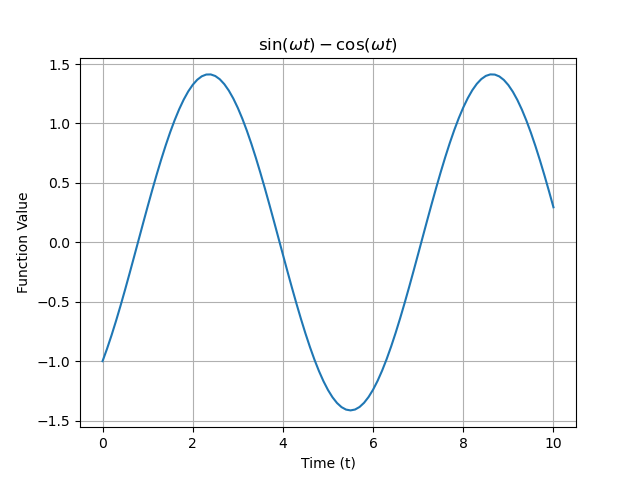
\includegraphics[width=\columnwidth]{ncert-physics/11/14/4/figs/11.14.4 f1.png}
    \caption{$\sin(2\pi f t)- \cos(2\pi f t)$}
    \label{fig:11.14.4.1}
\end{figure}
 \begin{figure}[h!]
    \centering
    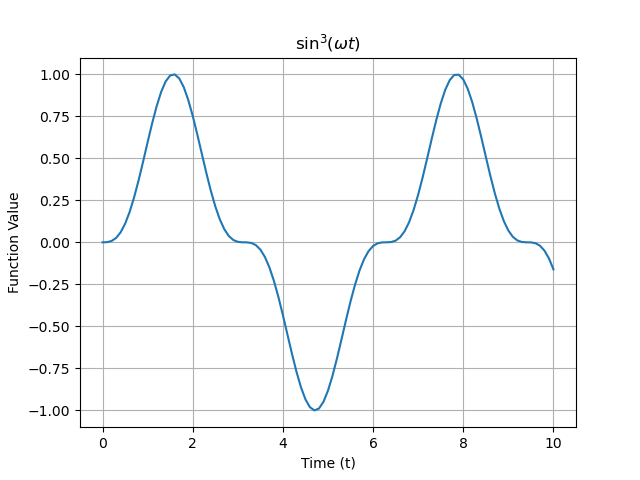
\includegraphics[width=\columnwidth]{ncert-physics/11/14/4/figs/11.14.4 f2.png}
    \caption{$\sin^3(2\pi f t)$}
    \label{fig:11.14.4.2}
\end{figure}
\newpage
\begin{figure}[h!]
    \centering
    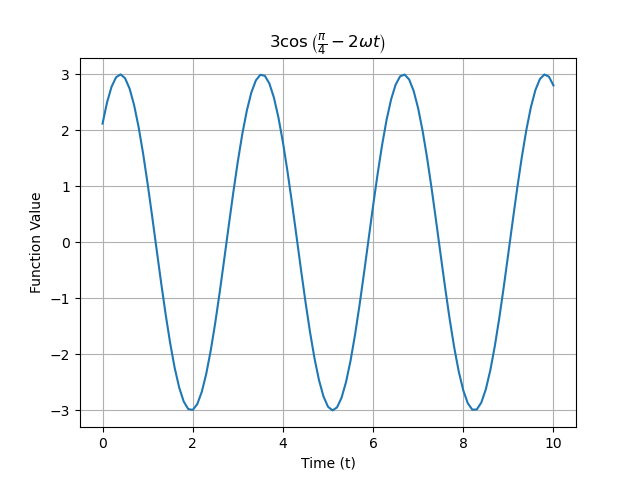
\includegraphics[width=\columnwidth]{ncert-physics/11/14/4/figs/11.14.4 f3.png}
    \caption{$3\cos\brak{\frac{\pi}{4}- 4\pi f t}$}
    \label{fig:11.14.4.3}
\end{figure}
\begin{figure}[h!]
    \centering
    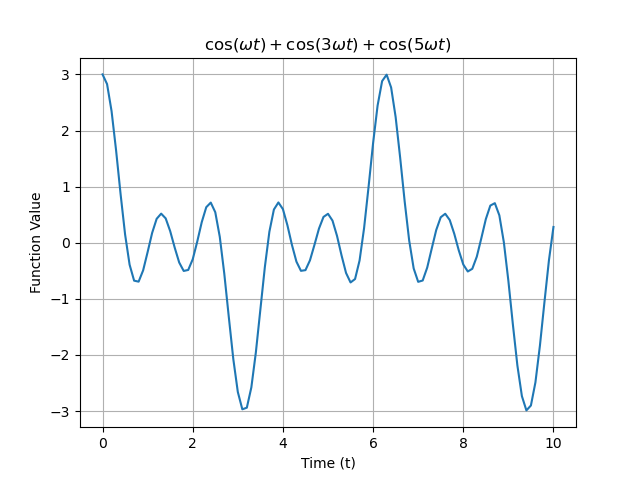
\includegraphics[width=\columnwidth]{ncert-physics/11/14/4/figs/11.14.4 f4.png}
    \caption{$\cos(2\pi f t)+\cos(6\pi  f t)+\cos(10\pi  f t)$}
    \label{fig:11.14.4.4}
\end{figure}
\begin{figure}[h!]
    \centering
    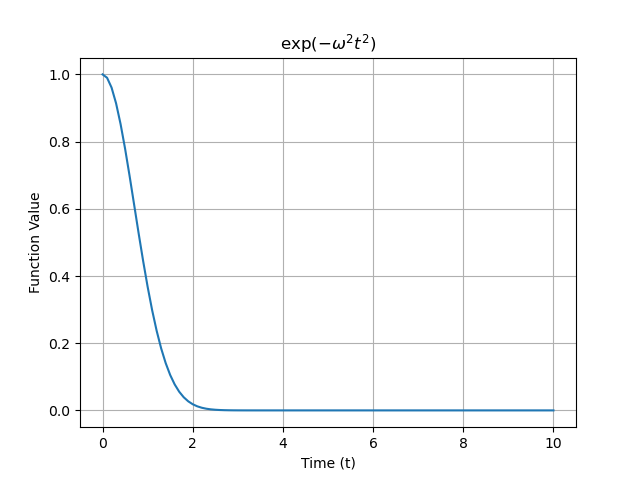
\includegraphics[width=\columnwidth]{ncert-physics/11/14/4/figs/11.14.4 f5.png}
    \caption{$exp^{\brak{-(2\pi ft)^2}}$}
    \label{fig:11.14.4.5}
\end{figure}
\begin{figure}[h!]
    \centering
    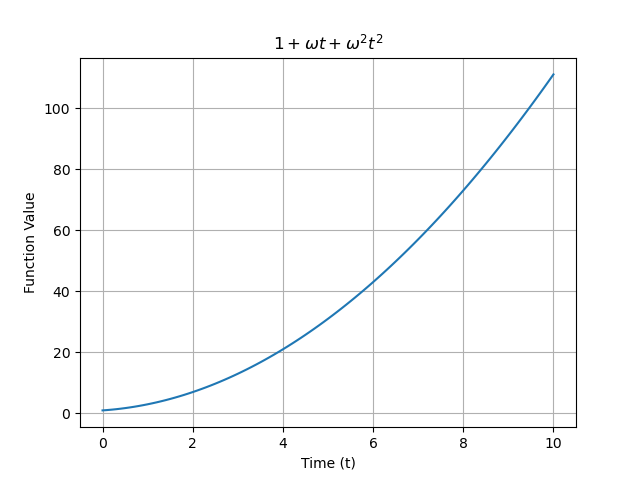
\includegraphics[width=\columnwidth]{ncert-physics/11/14/4/figs/11.14.4 f6.png}
    \caption{$1+2\pi f t+(2\pi f t)^2$}
    \label{fig:11.14.4.6}
\end{figure}
%\end{document}

 \pagebreak

 \item A metre-long tube open at one end, with a movable piston at the other end, shows resonance with a fixed frequency source (a tuning fork of frequency $340$ Hz) when the tube length is $25.5$ cm or $79.3$ cm. Estimate the speed of sound in air at the temperature of the experiment. The edge effects may be neglected.\\
 \solution
 \pagebreak
\item In a double-slit experiment the angular width of a fringe is found to
be $0.2^\circ$ on a screen placed 1 m away. The wavelength of light used is
600 nm. What will be the angular width of the fringe if the entire
experimental apparatus is immersed in water? Take refractive index
of water to be $\frac{4}{3}$
\solution
\pagebreak
\item An air chamber of volume V has a neck area of cross section a into which a ball of mass m just fits and can move up down without any friction. Show that when the ball is pressed down a little and released, it executes SHM. Obtain an expression for the time period of oscillations assuming pressure-volume variations of air to be isothermal.
\solution
\pagebreak

\item
(a) The refractive index of glass is $1.5$. What is the speed of light in
glass?(Speed of light in vacuum is $3.0\times 10^{8} m s^{-1}$) \\
\\
(b) Is the speed of light in glass independent of the colour of light? If
not, which of the two colours red and violet travels slower in a
glass prism?\\
\solution
\pagebreak
\item
The motion of a particle executing simple harmonic motion is described by the
displacement function, $x(t)$ = $A$ $cos$ ($\omega$$t$ +$\phi$).
If the initial $(t = 0)$ position of the particle is $1 cm$ and its initial velocity is $\omega\quad cm/s$, what are its amplitude and initial phase angle ? The angular frequency of the particle is $\pi\quad s^{-1}$. If instead of the cosine function, we choose the sine function to describe the SHM : $x$ = $B$ $sin$ ($\omega$$t$ +$\alpha$), what are the amplitude and initial phase of the
particle with the above initial conditions.\\
\solution
\pagebreak

\item A stone dropped from the top of a tower of height $300$ m splashes into the water of a pond near the base of the tower. When is the splash heard at the top given that the speed of the sound in air is $340$ m $s^{-1}$.(g=$9.8$ m $s^{-2}$)\\
\solution
\pagebreak

\item Monochromatic light of wavelength 589nm is incident from air on a
water surface. What are the wavelength, frequency and speed of\\
(a) Reflected light?\\
(b) refracted light? Refractive index of water is 1.33.\\
\solution
\pagebreak
\item A bat emits ultrasonic sound of frequency $1000 kHz$ in air. If the sound meets a water surface, what is the wavelength of\\[0pt] \brak a the reflected sound \\[0pt]
\brak{b} the transmitted sound?\\
Speed of sound in air is $340 ms^{-1}$ and in water is $1486 ms^{-1}$.\\
\solution
\pagebreak

\item A pipe 20 cm long is closed at one end. Which harmonic mode of the pipe is

resonantly excited by a 430 Hz source ? Will the same source be in resonance with

the pipe if both ends are open? (speed of sound in air is 340 m $s^{–1}$).\\
\solution
\pagebreak

\item Figures correspond to two circular motions. The radius of the circle, the period of revolution, the initial position and the sense of revolution(i.e. clockwise or anti-clockwise) are indicated on each figure. Obtain the corresponding simple harmonic motions of the x-projections of the radius vector of resolving particle P in each case.

\begin{figure}[H]
    \centering
    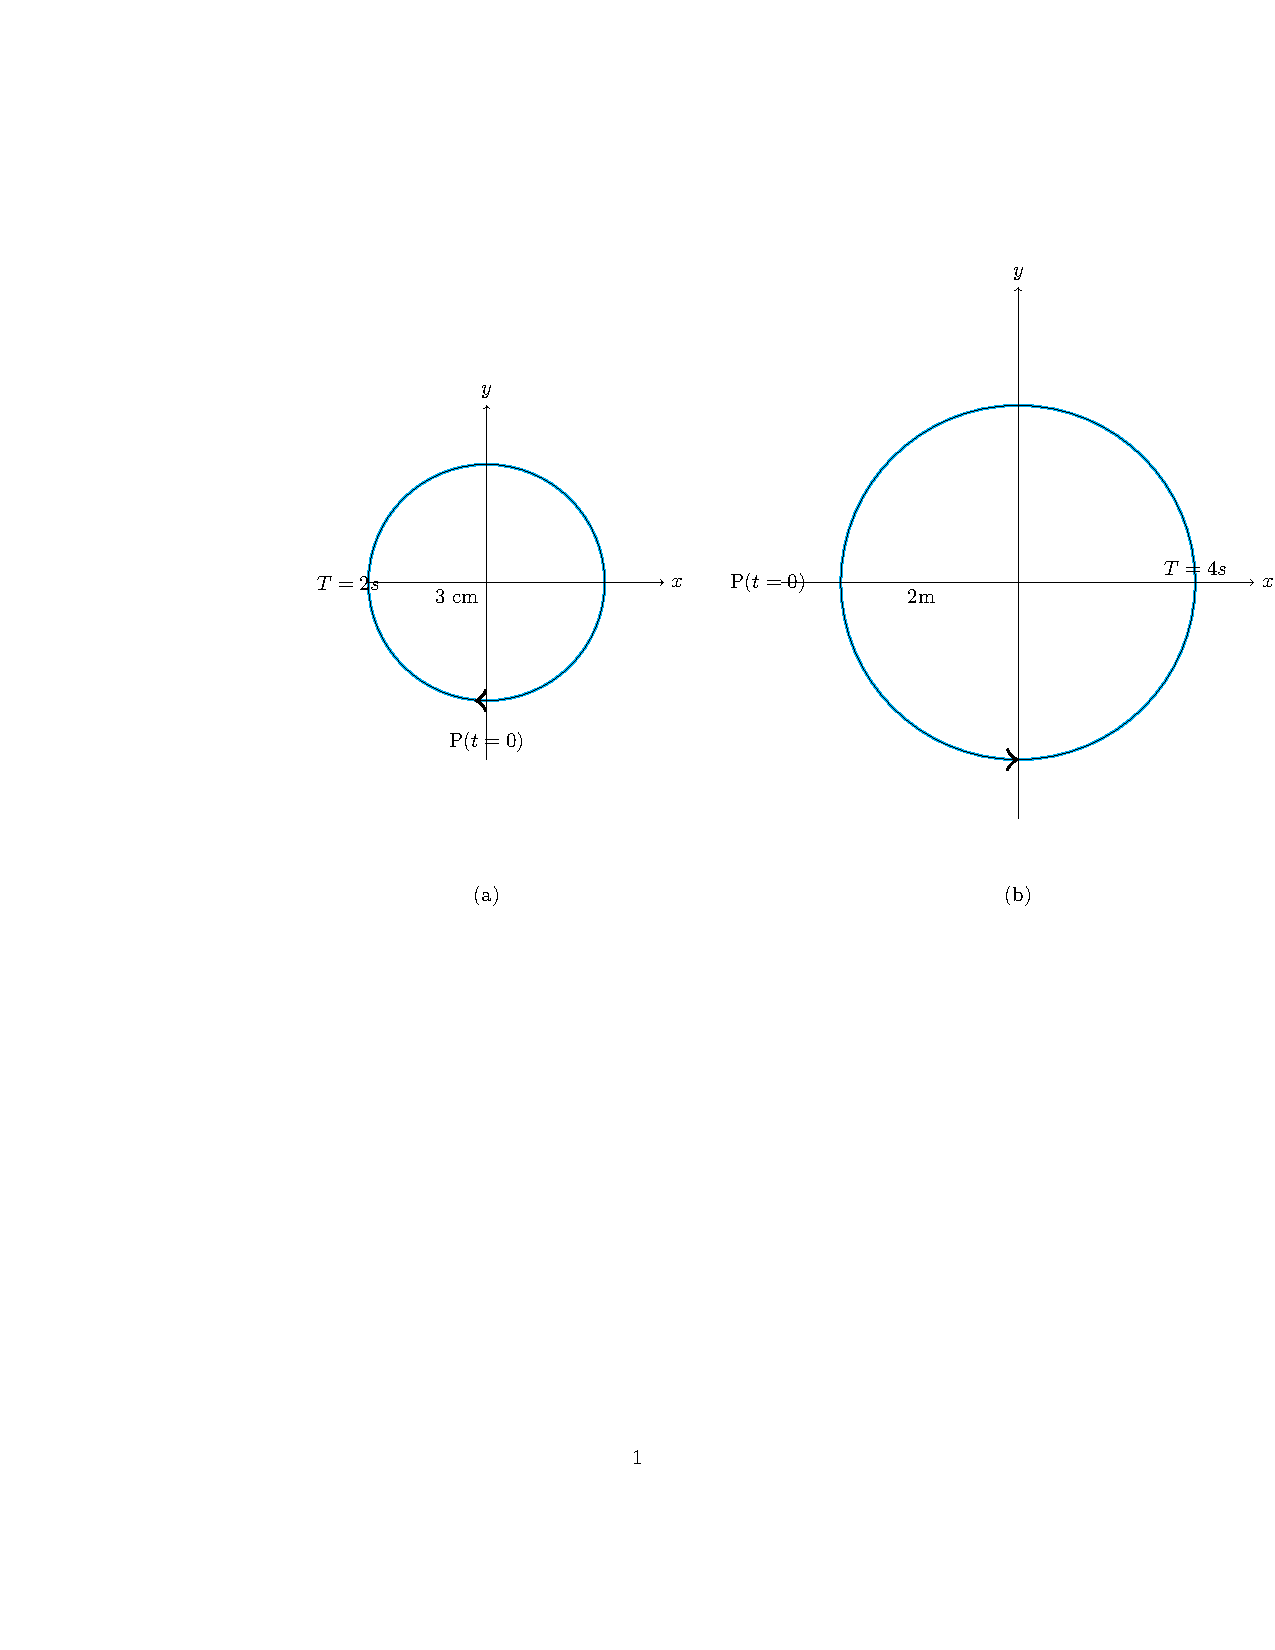
\includegraphics[width=\textwidth]{ncert-physics/11/14/11/codes/qfig.pdf}
\end{figure}
\solution
\pagebreak

\item A steel rod $100$cm long is clamped at its middle. The fundamental frequency of the longitudinal vibrations of the rod are given to be $2.53$kHz. What is the speed of sound in steel? \\
\solution
\pagebreak

\item A train, standing in a station yard, blows a whistle of frequency $400 \, \text{Hz}$ in still air. The wind starts blowing in the direction from the yard to the station with a speed of $10 \, \text{m/s}$. What are the frequency, wavelength, and the speed of sound for an observer standing on the station's platform? Is the situation exactly identical to the case when the air is still and the observer runs towards the yard at a speed of $10\, \text{m/s}$? The speed of sound in still air can be taken as $340\, \text{m/s}$.\\
\solution
\pagebreak

\item A radio can tune in to any station in the 7.5 MHz to 12 MHz band. What is the corresponding wavelength band?\\
\solution
\pagebreak

\item A travelling harmonic wave on a string is described by $$ y(x,t) = 7.5 \sin(0.0050x + 12t + \frac{\pi}{4}) $$
\begin{enumerate}
    \item[(a)] What are the displacement and velocity of oscillation of a point at $x = 1\,\text{cm}$ and $t = 1\,\text{s}$? Is this velocity equal to the velocity of wave propagation?
    
    \item[(b)] Locate the points on the string which have the same transverse displacements and velocity as the point at $x = 1\,\text{cm}$ at $t = 2\,\text{s}$, $t = 5\,\text{s}$, and $t = 11\,\text{s}$.
\end{enumerate}
\solution
\pagebreak
\end{enumerate}
